\documentclass[11pt,modernstyle]{thesis}
\usepackage{graphicx}
%\usepackage[maxbibnames=1, style=phys, backend=bibtex]{biblatex}
%\addbibresource{myref.bib}
\usepackage{lineno}
\usepackage{amsmath}
\usepackage{subfig}
\usepackage{setspace}
\usepackage{cancel}

\title{Search for supersymmetry in diphoton final states with the CMS detector}
\author{Matthew Lawrence Joyce}

\doublespacing
\begin{document}
	\maketitle
	\begin{abstract}
		This document presents a search for new physics having final states with two photons and missing transvers energy.  Data from proton-proton collisions with a center of mass energy of $\sqrt{s}=13$ TeV were used.  Said data was collected at the CERN LHC in the years 2016-2018 and make up a total integrated luminosity of 137 fb$^{-1}$.  Interpretation of the results was done in the context of gauge mediated supersymmetry breaking or more specifically the T5gg and T6gg simplified models.  The T5gg model is one where gluino pairs are produced which yield neutralinos which then each decay into a gravitino and a photon.  In the T6Wg model squark pairs are produced which yield neutralinos and then, as in the T5Wgg, each neutralino decays to a gravitino and a photon.  The gravitino would escape the detector undetected and therefore lead to a final state with missing transverse energy and two photons.  No significant excess was observed above the expected standard model backgrounds.  Lower limits were placed on the masses of the squarks and gluinos in the context of gauge mediated supersymmetry breaking.  Models with squark masses below -----  TeV were excluded at a 95\% confidence level as were models with gluino masses below ---- TeV.
	\end{abstract}
	\tableofcontents
	\listoffigures
	\listoftables
	\begin{linenumbers}	
	\chapter{The Standard Model of Particle Physics}

\section{The Standard Model}

The Standard Model (SM) of particle physics is a Lorentz-invariant quantum field theory (QFT) that describes the dynamics of elementary particles.  Three critical developments leading to the formation of the SM, as described by Steven Weinberg\cite{Weinberg:2004kv}, were the quark model proposed by Gell-Mann\cite{GellMann:1964nj} and Zweig\cite{Zweig:1964jf} in 1964, the idea of gauge symmetry by Yang and Mills\cite{Yang:1954ek} in 1954, and the notion of spontaneous symmetry breaking proposed by Goldstone\cite{Goldstone:1961eq} in 1961.  This ultimately led to the SM in its current form as a non-Abelian gauge theory with the symmetry group
\begin{equation}
	\label{equation:gaugesymmetry}
	G_{SM} = SU(3)_C \otimes SU(2)_L \otimes U(1)_Y
\end{equation}
where $SU(3)_C$ is responsible for strong interactions and $SU(2)_L \otimes U(1)_Y$ is responsible for unified electromagnetic and weak interactions, also known as electroweak interactions.

Associated with each of these symmetry groups is a set of massless spin-1 vector fields called gauge bosons.  These are listed in Table \ref{table:BosonFields} along with the associated charge or generator for that group.  There are eight such gauge bosons in $SU(3)_C$ called gluons $G_\mu^{1,...,8}$.  There are three gauge bosons $W_\mu^{1,2,3}$ in $SU(2)_L$ and one gauge boson $B_\mu$ in $U(1)_Y$.  The gauge bosons mediate the interactions between spin-1/2 fields $\psi$ called fermions.  At this point it's worth noting that the $W$ and $B$ gauge fields are not observable bosons, but are mixed by electroweak symmestry breaking to produce observable bosons.  The details of this will be covered in Section \ref{section:EWSB}.

There are twelve fermion fields which can be split into six lepton fields and six quark fields.  Both quarks and leptons are comprised of three generations.  For quarks there are three "up-type" quarks (up $u$, charm $c$, and top $t$) and three "down-type" quarks (down $d$, strange $s$, and bottom $b$).  The lepton fields are electron $e$, muon $\mu$, tau $\tau$, and three neutrino fields $\nu_e$, $\nu_\mu$, and $\nu_\tau$.  The fermion fields and their representations under $G_{SM}$ are listed in Table \ref{table:FermionTable}.  Each fermion field can be expressed in terms of left and right chirality fields, which are represented by a doublets $\psi_L$ in the left-handed case and singlets $\psi_R$ in the right-handed case with
\
\begin{eqnarray}
	\psi = \psi_R + \psi_L \\
	\psi_R = \frac{1}{2}(1+\gamma^5)\psi \\
	\psi_L = \frac{1}{2}(1-\gamma^5)\psi  
\end{eqnarray}

The SM also contains a complex scalar doublet field $\phi$ called the Higgs field in honor of Peter Higgs, who was among one of the physicists who proposed its existence in 1964 \cite{Higgs:1964pj}.  

\begin{table}[h!]
	\centering
	\caption{Boson fields in the SM}
	\begin{tabular}{|c|c|c|}
		\hline
		Symbol & Associated Charge & Symmetry group \\
		\hline
		\hline
		$B_\mu$ & weak hypercharge $Y$ & $U(1)_Y$\\
		\hline
		$G_{\mu}^{1,...,8}$ & color $C=(r,g,b)$ & $SU(3)_C$ \\
		\hline
		$W_{\mu}^{1,2,3}$ & weak isospin $T_3$ & $SU(2)_L$ \\
		\hline
	\end{tabular}
	\label{table:BosonFields}
\end{table}


%\begin{table}
%	\centering
%	\caption{Fermion fields in the SM.  }
%	\begin{tabular}{|c|c|c|}
%		\hline
%		Name & Symbol & \vbox{\hbox{\strut Representation under} \hbox{\strut $SU(3)_C, SU(2)_L, U(1)_Y$}} \\
%		\hline
%		\hline
%		Quarks & \vbox{\hbox{\strut($u_L$ $d_L$)} \hbox{\strut $u_{R}^\dagger$} \hbox{\strut $d_{R}^\dagger$}} & \vbox{\hbox{\strut (3, 2, $\frac{1}{6}$)}\hbox{\strut (3, 1, $-\frac{2}{3}$)}\hbox{\strut (3, 1, $\frac{1}{3}$)}} \\
%		\hline
%		Leptons & \vbox{\hbox{\strut($\nu$ $e_L$)}\hbox{\strut $e_{R}^\dagger$}} & \vbox{\hbox{\strut (3, 2, $-\frac{1}{2}$)} \hbox{\strut (1, 1, 1)}} \\
%		\hline
%	\end{tabular}
%	\label{table:FermionFields}
%\end{table}

\begin{table}
	\centering
	\caption{Fermions in the SM.  The first two numbers listed in the third column give the supermultiplet representation under $SU(3)_C$ and $SU(2)_L$ respectively.  A \textbf{1} means that it is not charged under that group and therefore will not couple to the associated force.  A \textbf{3} as the first number means that it has color charge and couples to the strong force.  A \textbf{2} for the second number means that it has weak isospin and couples to the weak force. The third number gives the value of the weak isospin.  Adjoint representation is specified by the presence of a bar over the number.}
	\begin{tabular}{|l|c|c|}
		\hline
		Name & Notation & \vbox{\hbox{\strut Representation under} \hbox{\strut $SU(3)_C \otimes SU(2)_L \otimes U(1)_Y$}} \\
		\hline
		\hline
		\vbox{\hbox{\strut Left-handed} \hbox{\strut quark doublet}} & 
		$
		\left(
		\begin{array}{c}
			u_L \\
			d_L \\
		\end{array}
		\right)
		$, 
		$
		\left(
		\begin{array}{c}
			c_L \\
			s_L \\
		\end{array}
		\right)
		$, 
		$
		\left(
		\begin{array}{c}
			t_L \\
			b_L \\
		\end{array}
		\right)
		$
		& (3, 2, $\frac{1}{6}$) \\
		\hline
		\vbox{\hbox{\strut Right-handed} \hbox{\strut up-type quark singlet}} & $u_R^\dagger$, $c_R^\dagger$, $b_R^\dagger$ & ($\bar{3}$, 1, -$\frac{2}{3}$) \\
		\hline
		\vbox{\hbox{\strut Right-handed} \hbox{\strut down-type quark singlet}} & $d_R^\dagger$, $s_R^\dagger$, $t_R^\dagger$ & ($\bar{3}$, 1, $\frac{1}{3}$) \\
		\hline
		\vbox{\hbox{\strut Left-handed} \hbox{\strut lepton doublet}} & 
		$
		\left(
		\begin{array}{c}
			\nu_{eL} \\
			e_L \\
		\end{array}
		\right)
		$, 
		$
		\left(
		\begin{array}{c}
			\nu_{\mu L} \\
			\mu_L \\
		\end{array}
		\right)
		$, 
		$
		\left(
		\begin{array}{c}
			\nu_{\tau L} \\
			\tau_L \\
		\end{array}
		\right)
		$
		& (1, 2, -$\frac{1}{2}$) \\
		\hline
		\vbox{\hbox{\strut Right-handed} \hbox{\strut charged lepton singlet}} & $e_R^\dagger$, $\mu_R^\dagger$, $\tau_R^\dagger$ & ($\bar{1}$, 1, 1) \\	
		\hline	
	\end{tabular}
\label{table:FermionTable}
\end{table}

The strong interaction is described by the theory of quantum chromodynamics (QCD).  The Lagrangian for the QCD interaction can be written as
\begin{equation}
	\mathcal{L}_{QCD} = \bar{\psi}(i\gamma^\mu D_\mu -m)\psi - \frac{1}{2}TrG_{\mu \nu}G^{\mu \nu}
	\label{equation:qcdlagrangian}
\end{equation}
where  
\begin{eqnarray}
	G_{\mu \nu} = \partial_\mu G_\nu - \partial_\nu G_\mu - ig_s[G_\mu , G_\nu] \\
	D_\mu = \partial_\mu - ig_sG_\mu
\end{eqnarray}
$g_s$ is related to the strong coupling constant, and $m$ is the fermion mass, which in this case must be a quark since they are the only fermions with color charge.

\section{Electroweak Symmetry Breaking} \label{section:EWSB}
A crucial feature of the SM is electroweak symmetry breaking.  The electroweak interaction, first proposed by Glashow, Weinberg, and Salam in the 60's, is the unified description of electromagnetic and weak interactions under the $SU(2)_L \otimes U(1)_Y$ symmetry.  The electromagnetic interaction is described by quantum electrodynamics (QED), which is an Abelian gauge theory under the $U(1)_{EM}$ symmetry group.  The gauge boson in QED is the photon and couples to electric charge $Q$. The QED Lagrangian is given by
\begin{equation}
	\mathcal{L}_{QED} = \bar{\psi}(i\gamma^\mu D_\mu -m)\psi - \frac{1}{4}F_{\mu \nu}F^{\mu \nu}
	\label{equation:qedlagrangian}
\end{equation}
where   
\begin{eqnarray}
	F_{\mu \nu} = \partial_\mu A_\nu - \partial_\nu A_\mu \\
	D_\mu = \partial_\mu + ieQA_\mu
\end{eqnarray}
and $A_\mu$ is the electromagnetic or photon field.

The Lagrangian for the unbroken $SU(2)_L \otimes U(1)_Y$ symmetry is given by
\begin{equation}
	\mathcal{L}_{EW} = \bar{\psi}i\gamma^\mu D_\mu \psi - Tr\frac{1}{8}W_{\mu \nu}W^{\mu \nu} - \frac{1}{4}B_{\mu \nu}B^{\mu \nu}
	\label{equation:ewlagrangian}
\end{equation}
where 
\begin{eqnarray}
	W_{\mu \nu} = \partial_\mu W_\nu - \partial_\nu W_\mu - ig_w[W_\mu , W_\nu] \\
	B_{\mu \nu} = \partial_\mu B_\nu - \partial_\nu B_\mu
\end{eqnarray}
with a separate fermion term for each field $\psi_R$ and $\psi_L$.  The covariant derivative $D_\mu$ is given by 
\begin{equation}
	D_\mu = \partial_\mu + ig_wT_iW_\mu^i + ig_Y \frac{Y}{2}B_\mu
\end{equation}
with $W_\mu^i$ and $T_i$ written in terms of raising and lowering operators 
\begin{eqnarray}
	W_\mu^\pm = \frac{1}{\sqrt{2}}(W_\mu^1\mp W_\mu^2) \\
	T^\pm = \frac{1}{\sqrt{2}}(T_1 \pm T_2) \\
	W_\mu^0 = W_\mu^3 \\
	T^0 = T_3
\end{eqnarray}
The neutral portion of the covariant derivative $ig_wT_3W_\mu^3 + ig_Y \frac{Y}{2}B_\mu $must contain the electromagnetic term $ieAQ$ for the electromagnetic interaction to be unified with the weak interaction, so the $W_\mu^3$ and $B_\mu$ fields need to linear combinations of the photon field $A_\mu$ and another field $Z_\mu$.  This relationship can be written in terms of the electroweak mixing angle $\theta_w$, also known as the Weinberg angle, as 
\begin{equation}
	\left(
	\begin{array}{c}
		A_\mu \\
		Z_\mu \\
	\end{array}
	\right)
	=
	\left(
	\begin{array}{cc}
		\cos\theta_W & \sin\theta_W \\
		-\sin\theta_W & \cos\theta_W
	\end{array}
	\right)
	\left(
	\begin{array}{c}
		B_\mu \\
		W_\mu^3 \\
	\end{array}
	\right)
\end{equation}
The weak isospin $T_3$ and weak hypercharge $Y$ can be related to the electric charge $Q$ with the Gell-Mann-Nishijima formula
\begin{equation}
	Y = 2(Q-T_3)
\end{equation}
and the coupling constants $g_w$, $g_Y$, and $e$ are related to the mixing angle by
\begin{eqnarray}
	e = g_w\cos\theta_W = g_Y\sin\theta_W \\
	\sin\theta_W = \frac{g_Y}{\sqrt{g_w^2 + g_Y^2}} \\
	\cos\theta_W = \frac{g_w}{\sqrt{g_w^2 + g_Y^2}}
\end{eqnarray}
At this point the $W_\mu^{1,2,3}$ and $B_\mu$ fields have been mixed to produce the observable fields $W_\mu^+$, $W_\mu^-$, $A_\mu$, and $Z_\mu$, but this is still inconsistent with experimental observations as these bosons and all of the fermions are still massless in this model.  In order to generate the masses while maintaining the renormalizability of the gauge theory the symmetry needs to be spontaneously broken.  This is done by the introduction of a complex scalar doublet field called the Higgs field which is expressed as
\begin{equation}
	\phi = 
	\left(
	\begin{array}{c}
		\phi^+ \\
		\phi^0
	\end{array}
	\right) = 
	\frac{1}{\sqrt{2}}\left(
	\begin{array}{c}
		\phi_1 + i\phi_2 \\
		\phi_3 + i\phi_4 
	\end{array}
	\right)
\end{equation}
where the fields $\phi_i$ are real scalar fields.  
The Lagrangian for the Higgs field is
\begin{equation}
	\mathcal{L}_{Hiigs} = (D_\nu\phi)^\dagger (D^\nu\phi) - V(\phi^\dagger \phi)
	\label{equation:higgsL}
\end{equation}
with the potential $V(\phi^\dagger \phi)$ being given by 
\begin{equation}
	V(\phi^\dagger \phi) = \mu^2\phi^\dagger \phi + |\lambda|(\phi^\dagger \phi)^2
\end{equation}
and the covariant derivative
\begin{equation}
	D_\nu = \partial_\nu - \frac{i}{2} g_wW_\nu^i \sigma_i - \frac{i}{2}g_YB_\nu
\end{equation}
Since $\mu^2<0$, this potential has the shape of a sombrero as is shown in Figure \ref{fig:higgspotential}.  The scalar fields have some positive vacuum expectation value (VEV) satisfying 
\begin{equation}
	\phi^\dagger \phi = v = \sqrt{-\frac{\mu^2}{\lambda}}
\end{equation}
at the minimum which allows us to write the ground state as
\begin{equation}
	\phi_{ground} = <0|\phi|0> = 
	\frac{1}{\sqrt{2}}
	\left(
	\begin{array}{c}
		0 \\
		v
	\end{array}
	\right)
\end{equation}
Expanding the Higgs field about it's minimum as 
\begin{equation}
	\phi_{ground} \rightarrow \phi(x) = \frac{1}{\sqrt{2}}e^{i\sigma_\alpha \theta^\alpha (x)}
	\left(
	\begin{array}{c}
		0 \\
		v + h(x)
	\end{array}
	\right), \alpha= 1,2,3
\end{equation}
results in a massive field $h(x)$ and and three massless scalar fields, or Goldstone bosons, $\theta_{1,2,3}$ which represent degrees of freedom.  By then transforming into the unitary gauge we can remove the phase factor, thereby eliminating the explicit appearance of the three Goldstone bosons in the Lagrangian.  In gauging away the Goldstone bosons, the three degrees of freedom reappear as longitudinal polarization states of the $W^+$, $W^-$, and $Z$ bosons.  In other words, the $W$ and $Z$ bosons have become massive by "eating" the Goldstone bosons.

\begin{figure}[h]
	\centering
	\includegraphics[width=0.7\linewidth]{Figures/higgspotential}
	\caption[Illustration of the Higgs potential for $\mu^2$ < 0]{The Higgs potential is shown as a function of the complex scalar field's real and imaginary parts. The balls illustrate that the stable vacuum state of nature is not located at $\phi$ = 0 because the symmetry at that point is spontaneously broken. Instead the stable vacuum state of nature is located somewhere along the circle of minimum potential. Reprint from \cite{Ellis:2011}}
	\label{fig:higgspotential}
\end{figure}


Writing the Lagrangian in Equation \ref{equation:higgsL} in terms of the physical $W$ and $Z$ fields and evaluating at the VEV gives 
\begin{equation}
	\begin{split}
	\mathcal{L}_{Higgs} = &\frac{1}{2}\partial_\nu h\partial^\nu h + \frac{1}{4}g_w^2W_\nu^+W^{-\nu}(v+h)^2 \\
	& + \frac{1}{8}\frac{g_w^2}{\cos^2\theta_W}Z_\nu Z^\nu (v+h)^2 - V[\frac{1}{2}(v+h)^2]
	\end{split}
\end{equation}
The $v^2$ terms give the $W$ and $Z$ boson masses and the $h^2$ term gives the mass of the Higgs boson as
\begin{eqnarray}
	M_W = \frac{1}{2}g_wv \\
	M_Z = \frac{1}{2}v\frac{g_w}{\cos\theta_W} = \frac{M_W}{\cos\theta_W} \\
	M_H = \sqrt{2}|\mu|
\end{eqnarray}
while the photon remains massless.

Charged leptons and quarks also acquire mass through Yukawa interactions via the Higgs mechanism.  For leptons the Yukawa interaction has the form of 
\begin{equation}
	\mathcal{L}_{Yukawa} = -G_e[\bar{e_R}\phi^\dagger\ell_L + \bar{\ell_L}\phi e_R]
\end{equation}
where 
\begin{equation}
	\ell_L = 
	\left(
	\begin{array}{c}
		\nu_{eL} \\
		e_L
	\end{array}
	\right)
\end{equation}
and $G_e$ is an arbitrary coupling parameter.  Note that this is the Yukawa term for the electron doublet.  The muon and tau doublets would have the same form.  Then using the unitary gauge version of $\phi$ we get 
\begin{eqnarray}
	\mathcal{L}_{Yukawa} = -\frac{G_e}{\sqrt{2}}(v + h)(\bar{e_L}e_R + \bar{e_R}e_L) \\
	= -\frac{G_ev}{\sqrt{2}}(\bar{e}e) -\frac{G_e}{\sqrt{2}}(h\bar{e}e)
\end{eqnarray}
where the electron mass is given by 
\begin{equation}
	m_e = \frac{G_ev}{\sqrt{2}}.
\end{equation}
Repeating the process for the second and third lepton generations gives the muon and tau masses as
\begin{equation}
	m_\mu = \frac{G_\mu v}{\sqrt{2}}, m_\tau = \frac{G_\tau v}{\sqrt{2}}
\end{equation}
Since there are no $\nu_R$ fields in the SM, neutrinos are not able to acquire mass the way charged leptons do.  

In order to generate quark masses for both the up and down-type quarks it's necessary to use $\phi$, which has $Y$ = 1, and the conjugate multiplet which is given by
\begin{equation}
	\tilde{\phi} = \left(
	\begin{array}{c}
	\phi^{0^*} \\
	-\phi^-
	\end{array}
	\right)
\end{equation}
and has $Y$ = -1.  The conjugate multiplet then, similar to $\phi$, breaks to 
\begin{equation}
	\tilde{\phi} \rightarrow \left(
	\begin{array}{c}
		v + h \\
		0
	\end{array}
	\right)
\end{equation}
The Yukawa term for the first generation quarks has the form
\begin{equation}
	\mathcal{L}_{Yukawa} = -G_d\bar{q_L}\phi d_R - G_u\bar{q_L}\tilde{\phi}u_R + h.c.
\end{equation}
where $G_d$ and $G_u$ are arbitrary coupling parameters and 
\begin{equation}
	q_L = \left(
	\begin{array}{c}
		u_L \\
		d_L
	\end{array}
	\right).
\end{equation}
Applying the broken $phi$ and $\tilde{\phi}$ gives us
\begin{equation}
	\mathcal{L}_{Yukawa} = -(m_d \bar{d}d + m_u\bar{u}u)(1 + \frac{h}{v})
\end{equation}
where the mass eigenstates are 
\begin{equation}
	m_q = \frac{G_qv}{\sqrt{2}}.
\end{equation}

It's worth noting that for each of these masses there is an arbitrary coupling parameter ($G_q$, $G_e$, $G_\mu$, and $G_\tau$).  This means that the values of the fermion masses are not predicted by SM, but these parameters are tuned to reflect observation.
%We can write the Lagrangian for the weak interaction as
%\begin{equation}
%	\mathcal{L}_{QED} = \bar{\psi}(i\gamma^\mu D_\mu -m)\psi - Tr\frac{1}{8}W_{\mu \nu}W^{\mu \nu}
%	\label{equation:qedlagrangian}
%\end{equation}


%Recall that there are three vector bosons ,$W_\mu^{1,2,3}$, associated with $SU(2)_L$ and one, $B_\mu$, associated with $U(1)_Y$.  

At this point we can summarize the particle content of the SM and their allowed interactions in a way that is seen in Figure \ref{fig:smcontent}.

\begin{figure}[h]
	\centering
	\includegraphics[width=1.0\linewidth]{Figures/SMcontent}
	\caption[Summary of content of the SM.]{Summary of particle content in the SM. Gray lines connecting groups of particles indicates allowed interactions. Self-coupling is indicated by a gray line connecting a particle to itself. The leptons and quarks are organized in columns corresponding to generation, which is specified at top, and rows corresponding to electric charge Q, which is listed to the left. Each particle's mass is listed beneath its name and symbol. It should be noted that neutrinos in the SM are still treated as massless leptons despite the fact that experimental evidence has established that at least two of the neutrinos are massive. Reprinted from \cite{Iiyama:2015nem}}
	\label{fig:smcontent}
\end{figure}


\section{Problems with the SM}
Though the SM has proven to be largely successful, there are still some limitations which must be addressed.  We can group these two categories.  The first of which is phenomena that have been observed experimentally yet are not explained by the SM.  The second is the question of why the SM requires a high degree of fine tuning of parameters to properly explain some phenomena.

\subsection{Missing from the SM}
The following is a description of some of the things that are missing from the SM.  This list is non-exhaustive but is meant to highlight the need for theories beyond the current scope of the SM in order to get a more complete understanding of all natural phenomena.

Perhaps the most noticeable omission in the SM is a description of the gravitational force.  While gravity is well understood over large distances by other means, attempts to construct a quantum theory of gravity have not been successful.  

Another issue is the lack of neutrino mass in the SM.  Neutrinos are left-handed without right-handed counterparts and therefore do not couple to the Higgs field which leaves them massless.  Experimental observations have shown that neutrinos undergo flavor oscillations which is only possible if they are massive.  The mechanism by which neutrinos gain their mass cannot be explained in the current framework of the SM.

The inability to explain the evidence of the presence of dark matter in the observable Universe is another shortcoming of the SM.  Studies of galactic rotation curves, the cosmic microwave background, and gravitational lensing, for example, indicate that dark matter comprises approximately 30\% of the energy density of the Universe is comprised of non-baryonic dark matter\cite{Darkmatter:2004pz}.  While there are a number of theories proposed that explain the existence of dark matter, there is currently no explanation in the SM.

\subsection{Fine tuning}
The issue of fine tuning revolves around the fact that there are at least 19 free parameters in the SM that are set by hand to seemingly unrelated and arbitrary values\cite{Ellis:2002wba}.  Having to tune these paramaters to have specific values in order to match observations is somewhat unsatisfying in a theoretical sense and begs the questions of whether there is some underlying mechanism that is causing them to take on these particular values.  The hierarchy problem is one such fine tuning issue which is related to the observed mass of the Higgs boson, measured to be 125 GeV by the CMS\cite{CMS:2012qbp} and ATLAS\cite{ATLAS:2012yve} experiments.  It's mass receives one-loop quantum corrections from all fermions which can be written as
\begin{equation}
	\Delta m_H^2 = -\frac{|\lambda_f|^2}{8\pi^2}\Lambda_{UV}^2 + ...
\end{equation}
where $\lambda_f$ is the Yukawa coupling and $\Lambda_{UV}$ is the ultraviolet cutoff which is energy up to which the SM is valid, which is taken to be at the Planck scale (10$^{19}$ GeV).  The quadratic dependence of the Higgs mass on $\Lambda_{UV}$ would make it much larger than the observed value.  Counter terms from all orders of perturbation theory would have to be extraordinarily precise and enormous in order to cancel the large corrections and keep the Higgs mass at its observed value.

\label{section:SMproblems}

	\chapter{Supersymmetry}

Supersymmetry (SUSY) is an elegant theory that deals with some of the SM issues described in Section \ref{section:SMproblems}.  One of the primary motivations of SUSY is to have a symmetric theory that connects fermions to bosons.  The SUSY operator $Q$ generates a transformation between boson and fermion states with 
\begin{eqnarray}
	Q\vert Boson \rangle = \vert Fermion \rangle, \\
	Q\vert Fermion \rangle =  \vert Boson \rangle
\end{eqnarray}
This means that for every SM boson there is a fermion superpartner and for every SM fermion there will be a boson superpartner.  It's important to note that the spins of the superpartners will differ from their SM counterparts by 1/2, while the other quantum numbers remain unchanged.  We now have a remedy for the hierarchy problem if we realize that the one-loop level corrections due to scalars is of the opposite sign for that of fermions and is given by
\begin{equation}
	\Delta m_H^2 = \frac{\lambda_s}{16\pi^2}\Lambda_{UV}^2 + ...
\end{equation}
where the coupling in this case is $\lambda_s$.  We can then cancel the troublesome one-loop corrections if we were to have two complex scalar fields for each SM fermion and the $\lambda_s = |\lambda_f|^2$.\cite{Martin:1997ns}

%There is a remedy for this if we realize that the one-loop level corrections due to scalars is of the opposite sign and is given by
%\begin{equation}
%	\Delta m_H^2 = \frac{\lambda_s}{16\pi^2}\Lambda_{UV}^2 + ...
%\end{equation}
%where the coupling in this case is $\lambda_s$.  That being said, the c

\subsection{Minimal Supersymmetric Standar Model (MSSM)}

In the SUSY framework the SM particles and their superpartners are arranged in supermultiplets\cite{Martin:1997ns}.  The SM fermions and their superpartners belong to chiral multiplets.  Each of which contains a Weyl fermion and a complex scalar field.  In these chiral multiplets, the names for each superpartner is that of its SM counterpart but this an 's' in front of it, i.e. 'selectron', 'stop squark', or more generally 'sleptons' and 'squarks'.  The 's' is meant to denote that it is a scalar superpartner.  The SM spin-1 gauge bosons and their superpartners belong to gauge supermultiplets.  Each of these contains a massless spin-1 boson and a massless Weyl fermion.  The Weyl fermions in the gauge supermultiplet are referred to with an 'ino' added as a suffix, i.e. 'wino', 'gluino', or more generally as 'gauginos'.  Table \ref{table:susyparticles} shows the particles in MSSM and their associated SM particles.
\begin{table}[h]
	\centering
	\caption{Summery of SM particles and superpartners}
	\begin{tabular}{|l|c|c|l|c|c|}
		\hline
		\hline
		\multicolumn{2}{|c|}{SM particles} & Spin & \multicolumn{2}{|c|}{MSSM particles} & Spin \\
		\hline
		Quark & q & 1/2 & Squark & $\tilde{q}$ & 0 \\
		Lepton & l & 1/2 & Slepton & $\tilde{l}$ & 0 \\
		\hline
		Gluon & g & 1 & Gluino & $\tilde{g}$ & 0 \\
		B & B & 1 & Bino &$\tilde{B}$ & 1/2 \\
		W & W & 1 & Wino & $\tilde{W}$ & 1/2 \\
		Higgs & H & 0 & Higgsino & $\tilde{H}$ & 1/2 \\
		\hline	
	\end{tabular}
	\label{table:susyparticles}  
\end{table}
After electroweak symmetry breaking the neutral gauginos, $\tilde{W}_0$ and $\tilde{B}_0$, and the Higgsino form four mass eigenstates referred to as neutralinos $\tilde{\chi}_0$.

A new quantum number, \textit{R-parity}, is used in the MSSM.  It can written as
\begin{equation}
	P_R = (-1)^{3\cdot(B-L)+2s}
\end{equation}
where \textit{B} represents the baryon number, \textit{L} represents the lepton number, and \textit{s} gives the spin.  All SM particles have $P_R = +1$ and all superpartners have $P_R = -1$.  This means that if we conserve R-parity all SUSY particles must will be produced in even number, or in the case of a collider experiment they will be pair produced.  Conservation of R-parity also makes the lightest SUSY particle (LSP) completely stable making it a good candidate for dark matter.  From the standpoint of a collider experiment, the completely stable LSP will exit the detector without leaving a signal so long as it is electrically neutral.  This lack of signal will present in the form of an imbalance in the reconstructed momentum in the transverse plane of the detector.  The magnitude of this imbalance is called the missing transverse energy $E_T^{miss}$.

\section{Gauge-mediated supersymmetry breaking}

Superpartners and their SM counterparts would have the same masses if SUSY were an unbroken symmetry, but since there has yet to be any experimental evidence of SUSY at what should be detectable masses, it must be that SUSY is a broken symmetry.  In this analysis we will focus on the model of gauge-mediated supersymmetry breaking (GMSB) in which SUSY is spontaneously broken.  In this model the SUSY breaking occurs in a "hidden" sector and then the breaking is communicated to the "visible" sector by messenger particles via SM gauge interactions\cite{Martin:1997ns}.  

The lightest SUSY particle in GMSB is the gravitino $\tilde{G}$, which is the superpartner of the gravitino.  Since the gravitino is a spin-2 particle, this makes the gravitino spin-3/2.  The gravitino is significantly lighter than all of the other SUSY particles in this model and since it is only able to interact with SM particles gravitationally, it would leave the detector without depositing any energy.  The lightest neutralino is taken to be the next-to-lightest supersymmetric particle (NLSP) and we assume that this promply decays as $\tilde{\chi}_1^0 \rightarrow \gamma \tilde{G}$, $\tilde{\chi}_1^0 \rightarrow Z \tilde{G}$, or $\tilde{\chi}_1^0 \rightarrow H \tilde{G}$ of which the first has a branching ratio of over 90\% in most GMSB models\cite{Terwort:2008ii}.  In this analysis we assume a 100\% branching ratio for $\tilde{\chi}_1^0 \rightarrow \gamma \tilde{G}$.  

As strong productions are dominant at a proton-proton collider such as the LHC, the prevailing modes of SUSY production are gluino pair production and squark pair production.  These are the modes that we target in this analysis.  In particular this analysis looks at two simplified models, T5gg and T6gg.  In the T5gg simplified model gluino pairs are produced from the proton-proton collision.  The gluinos decay to quark-antiquark pairs and neutralinos.  Each neutralino then decays to a photon and a gravitino.  In the T6gg simplified model squark pairs are produced which then each decays to a quark or antiquark and a neutralino.  The neutralinos then each decay to a photon and a gravitino.

%This model assumes that this breaking occurs in a "hidden sector" and new chiral supermultiplets act as messengers that interact with the "visible sector" which is where SM particles and their superpartners reside.  



	\chapter{The Large Hadron Collider}

\section{scratch section to work out outline...}
First thing to do is introduce the LHC as the large hadron collider and mention where it is located.  Now I should give a brief overview of what it does.  Now I need to talk about how it does this.  That means I need to mention how the protons are accelerated.  Then I need to explain how we contain and collide them once they are accelerated.  This leads into talking about the tunnel and magnets used for steering the bunches.

\section{Introduction}
The Large Hadron Collider (LHC) is a 26.7 kilometer-long two-ring particle accelerator and collider located on the border of France and Switzerland at the European Organization for Nuclear Research (CERN).  During normal operations the LHC maintains two counter-rotating beams of proton bunches that collide at four interaction points (IP).  The ALICE (Point 2), ATLAS (Point 1), CMS (Point 5), and LHC-b experiments each have a detector at one of these interaction points as scene in Figure \ref{fig:lhcips} .  The CMS and ATLAS are general-purpose detectors while LHC-b specializes in beauty quark studies.  ALICE is a heavy-ion experiment which uses $^{208}Pb-p$ or $^{208}Pb-^{208}Pb$ collisions that can also be produced by the LHC.

\begin{figure}[h]
	\centering
	\includegraphics[width=0.7\linewidth]{Figures/LHC_IPs}
	\caption[LHC interaction points]{Interaction points of the LHC}
	\label{fig:lhcips}
\end{figure}


\section{Injector Chain}


\section{Tunnel and Magnets}


\section{Luminosity} 

	\chapter{Compact Muon Solenoid}

\section{scratch}
Mention the location of CMS.  Give an overview of what it was designed to do.  Find a nice way to say that there is a lot of shit coming from the interaction region and we have to sort through it.  We need to get charged particle momentum and energy, electromagnetic energy, 

\section{Introduction}
About 100 meters below the town of Cessy, France at Point 5 is the Compact Muon Solenoid (CMS).  The CMS is a general purpose detector weighing 14,000 tonnes with a length of 28.7 meters and a 15.0-meter diameter that was designed to accurately measure the energy and momentum of particles produced in the proton-proton or heavy-ion collisions at the LHC \cite{Collaboration_2008}.  A perspective view of of the detector is shown in Figure \ref{fig:cmsschematic}.  In order to get a full picture of what is being produced by the collisions the CMS detector must be able identify the resulting particles as well as accurately measure their energy and momentum.  For this reason the detector was designed to be a collection of specialized sub-detectors, each of which contributes data used in the reconstruction of a collision.  
\begin{figure}[h]
	\centering
	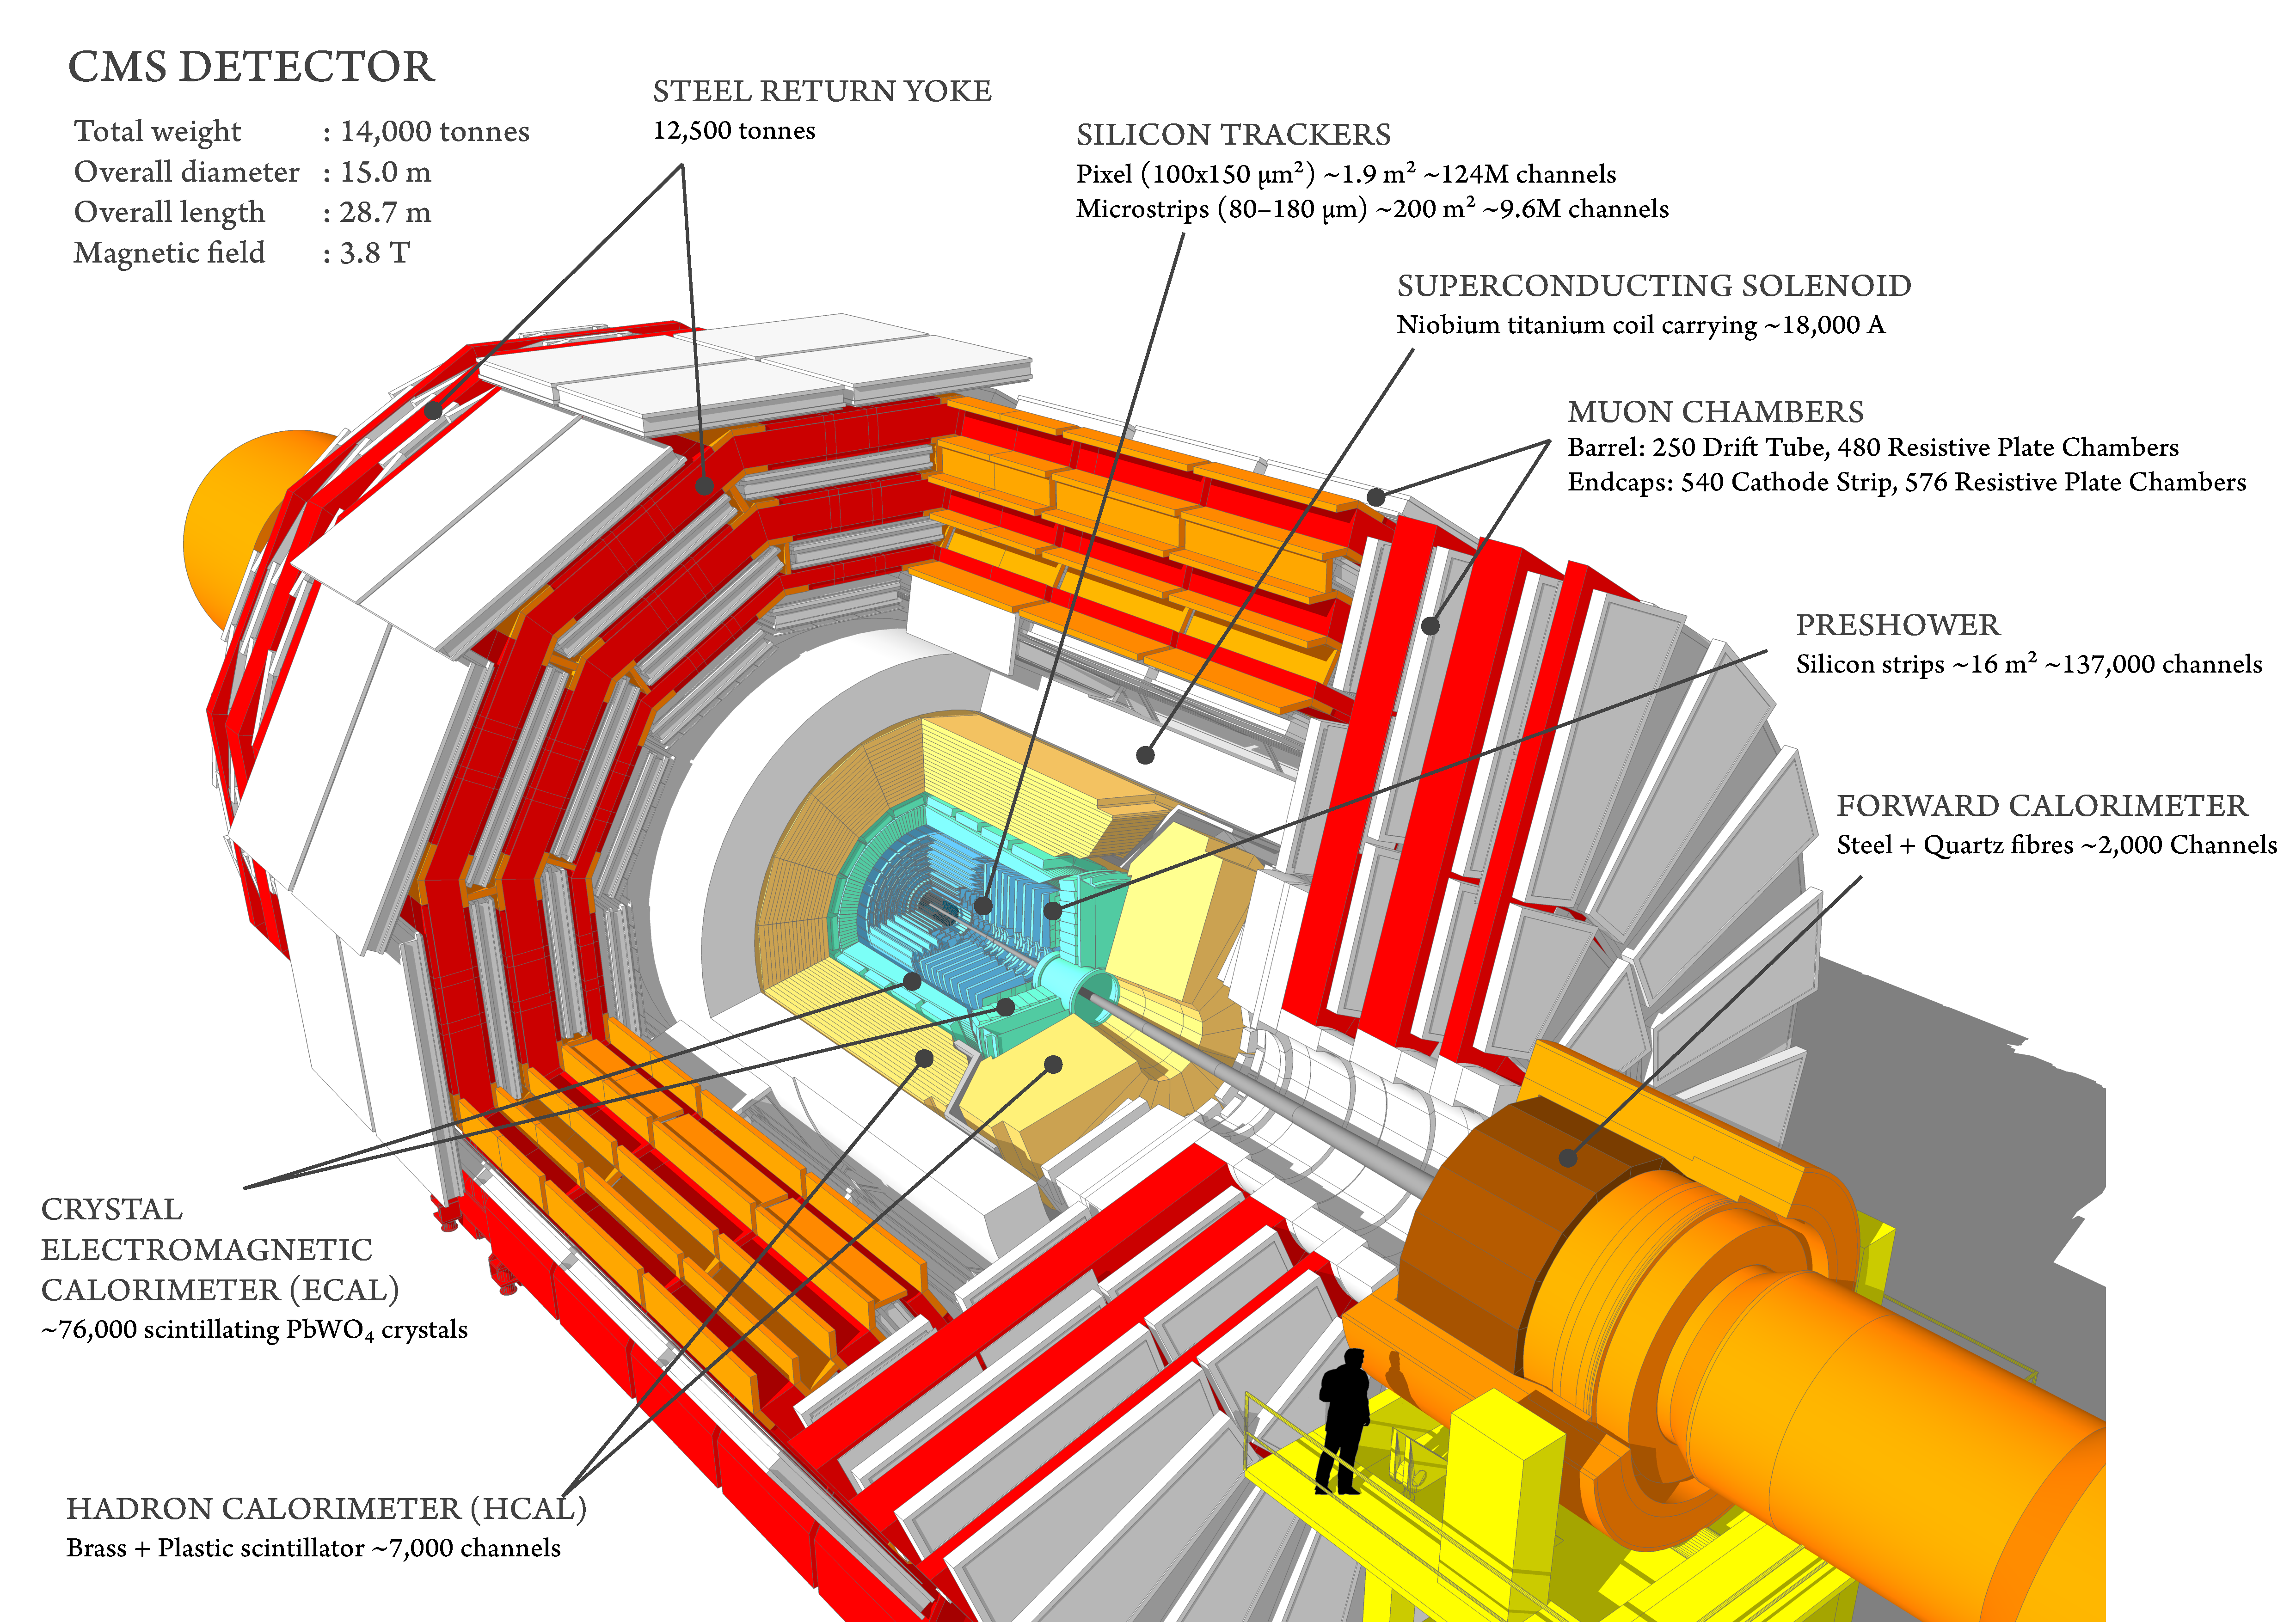
\includegraphics[width=0.7\linewidth]{Figures/cms_schematic}
	\caption{Schematic of CMS detector \cite{Sakuma_2014}}
	\label{fig:cmsschematic}
\end{figure}

At the heart of the CMS detector is a 3.8-Tesla magnetic field produced by a superconducting solenoid.  Inside the 6-meter diameter solenoid are three layers of sub-detectors.  These make up the inner detector and are, in order from innermost to outermost, the silicon tracker, the electromagnetic calorimeter (ECAL), and the hadronic calorimeter (HCAL).  Outside the solenoid is the muon system.  A transverse slice of the detector (Figure \ref{fig:cmsslicewhitecolourfrench291016}) shows the sub-detectors and how different types of particles interact with with them.  Table \ref{table:subdetsignals} shows a summary of which sub-detectors are expected to produce signals for different types of particles.

\begin{figure}[h]
	\centering
	\includegraphics[width=0.7\linewidth]{Figures/CMS_slice_white_colour_french_291016}
	\caption{Transverse slice of the CMS detector\cite{Barney:2628641}.}
	\label{fig:cmsslicewhitecolourfrench291016}
\end{figure}



\begin{table}[h]
	\centering
\begin{tabular}{|c|c|c|c|c|}
	\hline 
	Particle & Tracker & ECAL & HCAL & Muon \\ 
	\hline 
	Photons & No & Yes & No & No \\ 
	\hline 
	Electrons & Yes & Yes & No & No \\ 
	\hline 
	Hadrons (charged) & Yes & No & Yes & No \\ 
	\hline 
	Hadrons (neutral) & No & No & Yes & No \\ 
	\hline 
	Muons & Yes & No & No & Yes \\ 
	\hline 
	Invisible ($\nu$, SUSY, etc) & No & No & No & No \\ 
	\hline 
\end{tabular} 
\caption{Summary of signals expected for each particle type in each sub-detector}
\label{table:subdetsignals}
\end{table}


\section{Coordinate System}
The origin of the coordinate system used by CMS is centered at the nominal collision point in the center of the detector.  A right-handed Cartesian system is used with the x-axis pointing radially inward toward the center of the LHC ring, y-axis pointing vertically upward, and the z-axis pointing tangent to the LHC ring in the counterclockwise direction as viewed from above.  CMS also uses an approximately Lorentz invariant spherical coordinate system spanned by three basis vectors.  They are the transverse momentum $p_{T}$, pseudorapidity $\eta$, and azimuthal angle $\phi$.  The transverse momentum and azimuthal angle translate to the Cartesian system in the following ways using the x and y-components of the linear momentum:
\begin{equation}
p_{T} = \sqrt{(p_{x})^{2} + (p_{y})^{2}}
\end{equation}
\begin{equation}
\phi = tan^{-1}\frac{p_{y}}{p_{x}}
\end{equation}
while the pseudorapidity can be translated using the polar angle $\theta$ relative the positive z-axis as
\begin{equation}
\eta = -ln[tan\frac{\theta}{2}].
\end{equation}

\section{Tracker}

\section{Electromagnetic Calorimeter}

\section{Hadronic Calorimeter}

\section{Muon System}


	\chapter{CMS Trigger System}

When operating at nominal luminosity the LHC produces over 1 billion proton-proton collisions per second.  Finite computing speed and storage capacity limit the rate at which CMS can record events to be about 1 kHz \cite{Cadamuro:2017slr}.  Decreasing the rate from 1 GHz to 1 kHz is accomplished by using a two-level trigger system to quickly decide which events will be discarded and which will be recorded. The first stage is a hardware-based Level 1 (L1) trigger and the second stage is software-based High Level Trigger (HLT).  

\section{L1 trigger}
The L1 trigger decreases the rate by about six orders of magnitude from 1 GHz to 100 kHz by performing rough calculations on information from the ECAL, HCAL, and muon subsystems using field-programmable gate arrays (FPGAs).  The L1 trigger can be divided further into the calorimeter and muon triggers.  The schematic of the L1 trigger system in Figure \ref{fig:l1trigger} shows both the calorimeter and muon triggers.  The calorimeter trigger trigger uses information from the ECAL and HCAL subdetectors to construct photon, electron, and jet candidates in addition to quantities such as missing transverse momentum and total hadronic activity.  The muon trigger uses information from all three muon subsystems to construct muon candidates.  The outputs from the calorimeter and muon triggers goes into the Global Trigger (GT) which decides which events should be recorded and which are to be discarded \cite{Wittmann_2016}.

\begin{figure}
	\centering
	\includegraphics[width=1.0\linewidth]{Figures/L1Trigger}
	\caption{L1 trigger system.  Reprint from \cite{L1Triggerfigure:2013yva}}
	\label{fig:l1trigger}
\end{figure}

\subsection{Calorimeter trigger}
Trigger Primitives (TP) are the raw inputs from the ECAL and HCAL for the calorimeter trigger.  The TP, which contain information regarding the energy deposits in the calorimeters, are passed to the first layer of the calorimeter trigger.  This first layer consists of several FPGA cards that receive data from several bunch crossings, but are each mapped to a section of the detector.  This data is then passed on to the second layer in such a way that each FPGA in this layer will receive data for the entire calorimeter for each bunch crossing.  Candidate objects are then constructed and organized into a sorted list according to transverse momentum and passed on to the GT and the global muon trigger.


\subsection{Muon trigger}
TP for the muon trigger come from the three muon detectors, the CSCs, DTs, and RPCs.  These are then passed on to the first layer of the muon trigger (Muon Track-Finding Layer) where the TP are combined to reconstruct muon tracks for sections of $\phi$ for different regions of $|\eta|$.  The barrel track-finder for $|\eta|<0.83$, the endcap track-finder for $|\eta|>1.24$, and the overlap track-finder for $0.83<|\eta|<1.24$.  This data is passed on to the second layer where the sections of $\phi$ are merged and subsequently passed on to the global muon trigger where it is combined with the output from Calo Trigger Layer 2 to compute isolation.  The global muon trigger then combines the $\eta$ regions and passes a list of the top eight muon candidates to the GT.

\subsection{Global Trigger}
Final processing of the reconstructed objects and quantities constructed by the calorimeter and muon triggers is carried out by the GT.  L1 algorithms or "seeds" are implemented by the GT using these objects.  A full set of L1 seed is called a L1 menu and can be adjusted to meet the requirements of the CMS physics program.  Each L1 seed can be given a "prescale", which is an integer value $N$ that can be used to reduce the rate of a particular trigger path.  This is done by only applying the trigger to one out of $N$ events and can be used to take advantage of the current LHC running conditions.

\section{High Level Trigger}
Events that are accepted by the L1 trigger are passed on to the HLT which is based in software and is therefor capable of analyzing events with a higher degree of sophistication.  The HLT has access to information from the full detector and implements "paths" to select events of interest from those passing the L1 trigger.  Each HLT path is a set of criteria that is used to either accept or reject an event.  The full set of HLT paths is the HLT menu.  Each HLT path is "seeded" by one or more L1 seeds in order to decrease computing time.  That means that a given HLT path will only be processed if the L1 bits associated with its seed or seeds fire.  Each HLT path is assigned to a primary dataset depending on its general physics signature.  In the case of this analysis, the primary dataset used for signal events was DoubleEG for years 2016 and 2017.  This was merged into the EGamma dataset for 2018.  The SingleMuon dataset was used for trigger efficiency studies.  A list of the primary HLT used for each year along with its associated primary dataset is listed in Table \ref{table:HLTlist}.  The HLT path for 2016 is different because HLT\_DoublePhoton70 was not a part of the HLT menu until 2017.


\begin{table}[h!]
\centering
	\caption{Primary HLT}
	\begin{tabular}{|c|c|c|}
		\hline
		Year & HLT path & Primary dataset \\
		\hline
		2016 & HLT\_DoublePhoton60 & DoubleEG \\
		\hline
		2017 & HLT\_DoublePhoton70 & DoubleEG \\
		\hline
		2018 & HLT\_DoublePhoton70 & EGamma \\
		\hline
	\end{tabular}
\label{table:HLTlist}
\end{table}
\section{Trigger efficiency}

 
	\chapter{CMS Particle and Event Reconstruction}
After an event is chosen to be stored by the trigger system, the output from all of the sub-detectors is saved and recorded to disk as "RAW" data.  These data contain information about the response of each sub-detector, such as tracker hits and energy deposition in the calorimeters.  As was mentioned in Chapter 4, shown in Table \ref{table:subdetsignals} and Figure \ref{fig:cmsslicewhitecolourfrench291016}, the CMS was designed such that each type of particle resulting from the $pp$ collisions at the IP would leave a distinct signature in the sub-detectors.  This allows for the information to be reconstructed into lists of physics object candidates such as photons, electrons, muons, etc and quantities such as missing transverse momentum.  The particle flow (PF) algorithm performs this reconstruction by first building tracks and calorimeter clusters.  These two elements are the inputs to the reconstruction of the aforementioned physics object candidates using a "link" algorithm.

\section{Tracks}
A combinatorial track finder algorithm based on the Kalman filtering technique uses the hits in the silicon tracker to reconstruct tracks of charged particles \cite{Kalmantracking:1987fm}.  Each iteration of the algorithm is comprised of three steps:
\begin{itemize}
	\item Seed generation:  Find a seed consisting of two to three hits that is compatible with a track from a charged particle.
	\item Track finding: Use pattern recognition to identify any hits that are compatible with the trajectory implied by the seed generated in the first step.
	\item Track fitting: Determine the properties of the track, such as origin, trajectory, and transverse momentum by performing a global $\chi^2$ fit.
\end{itemize}

The first iteration uses stringent requirements on the seeds and the $\chi^2$ of the track fit to pick out isolated jets which have very high purity.  The hits associated with these high purity tracks are then removed to reduce the combinatorial complexity for subsequent iterations.  This allows successive iterations to identify less obvious tracks by progressively loosening criteria while the removal of previously associated hits mitigates the likelihood of fake tracks being built.  


\section{Calorimeter clusters}
Calorimeter clusters are constructed using energy deposition information from the calorimeters.  Clusters are formed by first identifying the seed cell (ECAL crystal or HCAL scintillating tile) that corresponds to the local maxima of an energy deposit that is above a given threshold.  Neighboring cells are then aggregated to grow topological clusters if their signals are above twice the standard deviation of the level of electronic noise.  

\section{Object identification}
At this point the tracks and calorimeter clusters are linked to form a PF block.  This linkage is done with an algorithm that quantifies the likelihood that a given track and cluster were results of the same particle.  As PF blocks are identified as object candidates they are removed from the collection prior to each subsequent iteration until all tracks and clusters have been assigned to a PF object candidate.  The following sections will outline how each of these PF objects is identified.
\subsection{Muons}
Muons are the easiest particle to identify, so they are the first objects reconstructed in the CMS.  PF Muons are classified in three categories depending on how their tracks are reconstructed:
\begin{itemize}
	\item Tracker muons:  Tracks reconstructed from the inner tracker having $p_T>0.5$ GeV and $|\vec{p}|>2.5$ GeV that, when propagated to the muon system, match at least one hit in the muon chambers.
	\item Stand-alone muons:  Tracks reconstructed only using hits in the muon system.
	\item Global muons:  Stand-alone muons that coincide with a track from the inner tracker.
\end{itemize}
After a muon is reconstructed it is given an identification or ID based on observables such as the $\chi^2$ of the track fit, how many hits were recorded per track, or how well the tracker and stand-alone tracks matched.  These IDs represent different working points (loose, medium, and tight) which correspond to increasing purity but decreasing efficiency as you move from loose toward tight.  
\subsection{Electrons}
The next objects reconstructed in the CMS are electrons.  Bremsstrahlung in the tracker layers causes substantial energy loss and changes in momentum which requires the use of a dedicated tracking algorithm.  In place of the Kalman filtering technique, a Gausian-sum filter (GSF) algorithm is used.  This algorithm uses a weighted sum of Gaussian PDFs which does a better job of modeling the Bremsstrahlung effects than the Kalman filtering technique which uses a single Gaussian PDF.  

PF ECAL clusters are regrouped by identifying a seed cluster then associating and adding clusters from Bremsstrahlung photons to form superclusters.  The schematic in Figure \ref{fig:electrontracking} shows how the Bremsstrahlung photons are emitted in directions tangent to the trajectory of the electron.  Electrons bending in the magnetic field causes spreading of PF ECAL clusters to typically occur along the $\phi$-direction.  Two approaches are used to associate the superclusters to GSF tracks.  One is the ECAL-driven method, which uses superclusters with $p_T > 4$ GeV as seeds for the GSF track finding algorithm.  This works well for high-$p_T$ isolated electrons because the bend radius is less severe which decreases the spread of the PF ECAL clusters. This results in more of the Bremsstrahlung radiation being recovered and correctly assoiated with an electron candidate.  The second approach is the tracker-driven method which uses tracks with $p_T > 2$ GeV as seeds that are propagated out to the surface of the ECAL and used for clustering.  This method works best with soft electrons like those in jets because it relies on the high granularity of the tracker to disentangle overlapping energy deposits in the ECAL. \cite{Electrontracking:2715343}

\begin{figure}[h]
	\centering
	\includegraphics[width=0.5\linewidth]{Figures/electrontracking}
	\caption{The Bremsstrahlung photons continue along a straight trajectory while the electron path is bent by the magnetic field.  This results in energy deposited in the calorimeter for such electrons to be spread out along the $\phi$-direction.}
	\label{fig:electrontracking}
\end{figure}

As a final step, a boosted decision tree (BDT) is used to discriminate between real and fake electrons.  The BDT is given variables associated with track-cluster matching, shower shape, and tracking.  The output score of the BDT is used to classify electrons into loose, medium, and tight working points which exhibit to the same purity and efficiency trends as the muon working points.

\subsection{Photons} 
Unlike electrons, photons typically deposit most of their energy in the ECAL without interacting with the tracker therefore their reconstruction is seeded from ECAL superclusters that do not have any GSF tracks associated with them.  When photons interact with the tracker material they convert into electron-positron pairs which follow bent trajectories due to the magnetic field prior to entering the ECAL.  This causes a spread of the energy deposition along the $\phi$-direction.  The goal of the clustering algorithm for photon reconstruction is to include all of the energy deposits of electrons resulting from photon conversions.  As with the calorimeter clustering algorithm, the photon clustering starts by identifying a local energy maxima as a seed crystal. In the EB a cluster is made up of several parallel strips of crystals $5\times1$ in $\eta \times \phi$.  The first strip has the seed crystal at its center.  Neighboring strips in the $\phi$-direction are added if they have energy above a threshold of 10 GeV but less than that of the subsequent strip with a maximum of 17 strips in a cluster.  In the EE, the seed cluster is $5\times5$ with adjacent $5\times5$ clusters being added if they meet the minimum energy requirement.

Converted and unconverted photons can be differentiated by looking at how the energy is distributed in a supercluster.  The variable $R_9$ is used for this purpose.  It is defined as the ratio of the energy in a $3\times3$ crystal array to the energy in the entire supercluster.  As the energy deposits resulting from converted electrons is more spread out they result in a lower $R_9$ value than unconverted photons.  A photon is candidate is considered to be unconverted when $R_9>0.93$.  

An important point regarding the clustering algorithm is that it does not differentiate between showers resulting from photons and those resulting from electrons.  This allows for electron from $Z\rightarrow ee$ events to be used as high purity samples to study analysis inputs and for defining control regions using electron in place of photons.


\subsection{Jets}
When quarks or gluons are produced they hadronize to make cone-shaped, collimated collections of particles called jets.  The jet clustering algorithm aims to combine these particles in order to accurately measure the kinematics of the initial gluon or quark.  The algorithm uses the two distance parameters
\begin{eqnarray}
	d_{ij} &=& min(k_{T_i}^{2p},k_{T_j}^{2p})\frac{\Delta R_{ij}^2}{R^2} \\
	d_{iB} &=& k_{T_i}^{2p}
\end{eqnarray}
where $d_{ij}$ is the distance between objects $i$ and $j$ and $d_{iB}$ is the distance between object $i$ and the beam $B$.  The transverse momentum of the object is $k_T$.  The parameter $p$ is set either -1, 0, or +1 to specify whether the anti-$k_T$, inclusive Cambridge/Aachen, or inclusive $k_T$ algorithm is used, respectively.  The value of $\Delta R_{ij}^2$ is defined as $(\eta_i-\eta_j)^2+(\phi_i-\phi_j)^2$ and $R$ is the distance parameter that defines the radius of the jet.

his analysis uses jets reconstructed from PF candidates using the anti-$k_T$ algorithm with $R= 0.4$, also known as AK4PFJets or just PFJets. The algorithm goes through the following steps:
\begin{enumerate}
	\item The smallest values of $d_{ij}$ and $d_{iB}$ are computed for all objects in the event.
	\item Objects $i$ and $j$ are merged into a single object if $d_{ij}<d_{iB}$.  
	\item Object $i$ is labeled as a jet and removed from the list if $d_{iB}<d_{ij}$. 
\end{enumerate}

Note for next time:  
Now talk about infrared and collinear safe.  Use Allie's thesis for guide.
Look at "recent thesis" for ECAL noise on 2017 data.
Should also do JEC and JER in here. 


\section{Missing transverse momentum}


	\chapter{Data Analysis}

\section{Overview}



This analysis is motivated by the GGM supersymmetry breaking scenario in which the strong production of either gluinos or squarks result in a final state containing two photons, jets, and missing transverse momentum.  Two example topologies are shown in Figure \ref{fig:susysignals}.  In the T5gg model, each of the produced gluinos decays to a neutralino which then decays to a photon and a gravitino.  Similarly, the T6gg model has each of the produced squarks decays to a neutralino which then decays to a photon and a gravitino.  In both cases the gravitino escapes the CMS without detection which manifests as missing transverse momentum.  

\begin{figure}[h]
	\centering
	\includegraphics[width=0.9\linewidth]{Figures/SUSYsignals}
	\caption{Two examples of GGM supersymmetry breaking processes resulting in final states conaining two photons and missing transverse momentum. The T5gg model (left) shows gluinos produced from $p-p$ collisions which subsequently result in two neutralinos, each decaying to a photon and a gravitino. The T6gg model (right) shows squarks produced from $p-p$ collisions following a similar decay chain.}
	\label{fig:susysignals}
\end{figure}


\section{Data}
This analysis was performed using 137 fb$^{-1}$ of data collected from the CMS detector during the time period commonly referred to as Run 2 which spans from  2016 to 2018.  The complete list of the datasets used can be found in Table \ref{table:DataSamples}.  The JSON files used to identify events passing all of the CMS offline data quality monitoring requirements are:

\begin{verbatim}
	Cert_271036 284044_13TeV_23Sep2016ReReco_Collisions16_JSON.txt
	Cert_294927 306462_13TeV_EOY2017ReReco_Collisions17_JSON_v1.txt 
	Cert_314472 325175_13TeV_PromptReco_Collisions18_JSON.txt 
\end{verbatim} 

\begin{table}[h!]
	\centering
	\caption{Data Samples}
	\begin{tabular}{|c|}
		\hline
		/DoubleEG/Run2016B-17July2018-ver2-v1 \\
		\hline
		/DoubleEG/Run2016C-17July2018-v1 \\
		\hline
		/DoubleEG/Run2016D-17July2018-v1 \\
		\hline
		/DoubleEG/Run2016E-17July2018-v1 \\
		\hline
		/DoubleEG/Run2016F-17July2018-v1 \\
		\hline
		/DoubleEG/Run2016G-17July2018-v1 \\
		\hline
		/DoubleEG/Run2016H-17July2018-v1 \\
		\hline
		/DoubleEG/Run2017B-31Mar2018-v1 \\
		\hline
		/DoubleEG/Run2017C-31Mar2018-v1 \\
		\hline
		/DoubleEG/Run2017D-31Mar2018-v1 \\
		\hline
		/DoubleEG/Run2017E-31Mar2018-v1 \\
		\hline
		/DoubleEG/Run2017F-31Mar2018-v1 \\
		\hline
		/EGamma/Run2018A-17Sep2018-v2 \\
		\hline
		/EGamma/Run2018B-17Sep2018-v1 \\
		\hline
		/EGamma/Run2018C-17Sep2018-v1 \\
		\hline
		/EGamma/Run2018D-22Jan2019-v2 \\
		\hline
	\end{tabular}
	\label{table:DataSamples}
\end{table}

\section{Monte Carlo samples}
Monte Carlo (MC) simulation were used to validate performance of the analysis on backgrounds, model background contributions, constructing a multivariate discriminant, and determining signal efficiencies.   The MC samples used for this analysis are listed in Table \ref{table:MCSamples}.
\begin{table}
	\centering
	\caption{Table of MC samples used.}
	\begin{tabular}{|l|l|}
		\hline
		Sample name & Purpose \\
		\hline
		\hline
		GJets & Training MVA discriminate for QCD background \\
		\hline
		ZGGToNuNuGG & Prediction of irreducible $Z\gamma \gamma \rightarrow \nu \nu \gamma \gamma$ background \\
		\hline
		ZGGToLLGG & Renormalization of $Z\gamma \gamma \rightarrow \nu \nu \gamma \gamma$ background \\
		\hline
		TTJets & Testing EWK background prediction method\\
		\hline
	\end{tabular}
	\label{table:MCSamples}
\end{table}

The distribution of pileup (PU) interactions produced in simulated events differs from data.  Since the presence of additional PU interactions affects many aspects of reconstruction, it's important for the PU to be properly simulated.  To correct for these differences between MC and data the simulated events are reweighted so that the PU profile in MC matches the profile in data.  In MC the PU is number of simulated vertices in an event while the PU in data is calculated by the method discussed in Section \ref{section:pucorrection}.  
  

\section{Object definitions}
The object candidates that are identified by the reconstruction algorithms are subject to further scrutiny in order to achieve optimal purities in the offline analysis.  

\subsection{Photons}
Photons are required to have $p_T>80$ GeV and meet the criteria prescribed by loose ID cuts derived by the $e/\gamma$ Physics Object Group (EGM POG).  The cut variables used to determine the photon ID are:

\begin{itemize}
	\item H/E - The ratio of the energy deposited in the HCAL tower that is directly behind the ECAL supercluster associated with the photon to the energy deposited in the ECAL supercluster.
	\item $\sigma_{i\eta i\eta}$ - The log-fractional weighted width of a shower in $i\eta$-space.  This variable is used to describe the shower shape or more specifically it provides a measure of the spread of the shower in the $\eta$-direction.  The log-fractional weight is the log of the ratio of energy deposited in a specific ECAL crystal versus the energy deposited in the associated $5\times 5$ supercluster.
	\item Particle Flow Charged Isolation - Sum of the $p_T$ of charged hadrons associated with the primary vertex within a cone of $0.02 < \Delta R < 0.3$ of the supercluster.
	\item Particle Flow Neutral Isolation - Sum of the $p_T$ of neutral hadrons associated with the primary vertex within a cone of $\Delta R < 0.3$ of the supercluster.
	\item Particle Flow Photon Isolation - Sum of the $p_T$ of photons within a cone of $\Delta R < 0.3$ of the supercluster.
\end{itemize}

All of the isolation variables listed above are corrected in order to remove pileup as described in Section \ref{section:pucorrection}.  Table \ref{table:looseIDPhotonreq} gives a summary of the pileup-corrected requirements for a loose ID photon.  The loose ID working point has an efficiency (background rejection) of $90.08\%$ ($86.25\%$) in the barrel and $90.65\%$ ($76.72\%$) in the end caps.  In addition to the $p_T$ and loose ID requirements, a photon must also pass a pixel seed veto (PSV).  This means that there is no pixel seed in the tracker matched to the photon.

\begin{table}[h]
	\centering
	\caption{Summary of loose ID photons cuts}
	\begin{tabular}{|l|l|l|}
		\hline
		Variable & Cut Value (Barrel) & Cut Value (Endcap) \\
		\hline
		H/E & 0.04596 & 0.0590 \\
		\hline
		$\sigma_{i\eta i\eta}$ & 0.0106 & 0.0272 \\
		\hline
		Charged Iso & 1.694 & 2.089 \\
		\hline
		Neutral Iso & $24.032 + 0.01512 p_{T\gamma} + 2.259\times 10^{-5}p^2_{T\gamma}$ & $19.722 + 0.0117 p_{T\gamma} + 2.3\times 10^{-5}p^2_{T\gamma}$ \\
		\hline
		Photon Iso & $2.876 + 0.004017 p_{T\gamma}$ & $4.162 + 0.0037 p_{T\gamma}$ \\
		\hline
	\end{tabular}
	\label{table:looseIDPhotonreq}
\end{table}

Photon ID efficiencies differ between data and MC, so when using a photon ID in MC samples we scale them by a "scale factor" (SF) in order to replicate detector efficiencies for that that particular ID.  The loose photon ID efficiency is measured using the tag-and-probe method on $Z\rightarrow ee$ events in both data and MC.  The probe is chosen to be one of the electrons while the other electron is used as the tag.  The ratio of how many probes pass the loose photon ID requirements and the total number of tag and probe pairs gives the efficiency $\epsilon$ for the loose photon ID.  We then define the SF as the data efficiency divided by the efficiency in MC or $SF = \frac{\epsilon_{data}}{\epsilon_{MC}}$.  Applying the SF to MC events essentially removes the MC efficiency and replaces it with the real detector efficiency to give
\begin{equation}
	N_{obs} = N_{gen}\cdot \epsilon_{MC}\cdot SF =  N_{gen}\cdot \epsilon_{MC}\cdot \frac{\epsilon_{data}}{\epsilon_{MC}} = N_{gen}\cdot \epsilon_{data}.
\end{equation}
Since this analysis requires two loose ID photons, the scale factor $SF$ is given by the product of scale factors for each of the two loose photons, $SF = SF_{\gamma1}\cdot SF_{\gamma2}$.  The scale factors for each year are shown in Figures \ref{fig:loosephotonsf2016}, \ref{fig:loosephotonsf2017}, and \ref{fig:loosephotonsf2018} in bins of photon $p_T$ and $\eta$ \cite{PhotonSF}.
\begin{figure}[h]
	\centering
	\includegraphics[width=1.0\linewidth]{Figures/LoosePhotonSF_2016}
	\caption[Scale factors for 2016 loose photon ID.]{The loose photon ID scale factors for 2016 in bins of photon $p_T$ and $\eta$}
	\label{fig:loosephotonsf2016}
\end{figure}
\begin{figure}[h]
	\centering
	\includegraphics[width=1.0\linewidth]{Figures/LoosePhotonSF_2017}
	\caption[Scale factors fo 2017 loose photon ID.]{The loose photon ID scale factors for 2017 in bins of photon $p_T$ and $\eta$.}
	\label{fig:loosephotonsf2017}
\end{figure}
\begin{figure}[h]
	\centering
	\includegraphics[width=1.0\linewidth]{Figures/LoosePhotonSF_2018}
	\caption[Scale factors for 2018 loose photon ID.]{The loose photon ID scale factors for 2018 in bins of photon $p_T$ and $\eta$.}
	\label{fig:loosephotonsf2018}
\end{figure}


\label{section:photondefinition}

\subsection{Electrons}
As mentioned earlier, the clustering algorithm doesn't differentiate between showers from photons and those from electrons.  In this analysis an electron is defined as an object that passes all of the photon requirements except for the PSV.  Inverting the pixel seed requirement while using the same ID criteria ensures that we have orthogonal selections while minimizing the bias potentially introduced by using control regions with electrons to model diphoton signal regions.  This essentially allows us to group photons and electrons together to be treated as electromagnetic objects and then splitting those objects into photon and electron objects depending on whether or not there is a pixel seed associated with it.


\subsection{Muons}
Muons are required to have $p_T > 30$ GeV, $|\eta|<2.4$, and pass the medium ID requirements listed below \cite{Sirunyan_2018}:
\begin{itemize}
	\item Must be identified by PF algorithm as either a tracker or a global muon.
	\item At least 80\% of the inner tracker layers traversed by a track must have recorded hits.
	\item If it's only reconstructed as a tracker muon, the muon segment compatibility must be > 0.451.
	\item If it's reconstructed as both a tracker and a global muon:
	\begin{itemize}
		\item the muon segment compatibility must be > 0.303
		\item the global fit must have a goodness-of-fit per degree of freedom  ($\chi^2$/dof) < 3
		\item the $\chi^2$ of the position match between standalone muon and the tracker muon must be < 12
		\item the kink-finding algorithm must give a maximum $\chi^2$ that is < 20
	\end{itemize}
\end{itemize}		
The types of muons (global, tracker, and standalone) are those described in Chapter \ref{section:muondefinitions}.  The medium ID criteria results in an efficiency of > 98\% for muons with $p_T > 20$ GeV \cite{MuonIDPerf}.

\subsection{Jets}
Jets are reconstructed using the anti-k$_T$ algorithm described in Chapter \ref{section:jetalgorithm} within a cone having radius $R = 0.4$.  

The nature of this reconstruction also labels the previously mentioned objects (photons, electrons, and muons) as jets so these need to be removed from the jet collection in order to leave us with only hadronic jets.  This process is called "cleaning" the jets. 

Still working on this section...

\label{section:jetdefinition}

\section{Event selection}
Candidate events are required to pass the following requirements:
\begin{itemize}
	\item Number of loose photons without a pixel seed requirement $\geq 2$
	\item Number of hadronic jets $\geq 2$
	\item Hard $E_T^{miss} \geq 130$ GeV
	\item Pass HLT
	\item Pass relevant event filters recommended by various POGs
\end{itemize}
The event filters mentioned above are designed to reject events with instrumental anomalies such as noise and beam backgrounds.  These filters are:
\begin{itemize}
	\item globalSuperTightHalo2016Filter
	\item HBHENoiseFilter
	\item HBHEIsoNoiseFilter
	\item eeBadScFilter
	\item BadChargedCandidateFilter
	\item BadPFMuonFilter
	\item CSCTightHaloFilter
	\item EcalDeadCellTriggerPrimitiveFilter
	\item ecalBadCalibReducedExtraFilter
	\item ecalBadCalibReducedFilter
	\item Good vertex filter (requiring at least one good reconstructed vertex)
\end{itemize}

\section{Backgrounds}
The sources of background in this analysis can be grouped into three categories.  In order of decreasing contribution they are mismeasured hadronic activity, electrons misidentified as photons, and standard model processes having final states with neutrinos and two photons.  In events with multiple jets, limitations on the jet energy resolution can give rise to an apparent imbalance in $p_T$ as is shown in Figure \ref{fig:fakemet}.  Such events are usually from quantum chromodynamics (QCD) processes.  In these cases jets can be misidentified as photons or there can be real photons being produced.  In both cases the result is the appearance of two photons accompanied by $E^{miss}_T$ which mimics our signal.  Given the large cross-section for QCD, this is the most significant background in this analysis.  The next background, resulting from the misidentification of electrons as photons, comes from electroweak (EWK) processes, in particular $W\gamma$ and $W + jets$ events where $W \rightarrow e\nu$.  Here the neutrino contributes real $E^{miss}_T$ while the fake photon allows this event to fulfill the diphoton requirement.  The final background is from $Z\gamma \gamma \rightarrow \nu \nu \gamma \gamma$ events, which exactly mimic our signal, and is modeled using simulation as it is irreducible.

\begin{figure}
	\centering
	\includegraphics[width=0.5\linewidth]{Figures/FakeMET}
	\caption{Mismeasurement of Jet3 results in an inbalance in the events transverse momentum.}
	\label{fig:fakemet}
\end{figure}

\subsection{Instrumental background}
The instrumental background is the contribution from events with spurious $E^{miss}_T$ due to mismeasured hadronic activity.  The vast majority of interactions produced from proton-proton collisions at the LHC are hadronically rich QCD events.  Aside from some very rare final states with heavy-flavor jets, these events do not include neutrinos, which are the only stable particles in the SM that pass through the CMS detector unobserved, and therefore exhibit little or no $E^{miss}_T$ at the parton level.  However, the measurements of final-state particles are made using the tracker and calorimeters which have finite energy and momentum resolution.  These limitations propagate into the calculation of $E^{miss}_T$ leading to an inequality between the real, parton level $E^{miss}_T$ in an event and the measured $E^{miss}_T$.  Since most of this background is comprised of QCD events, it is commonly referred to as the "QCD background" and those terms are used interchangeably in this thesis.  Modeling of this background was done using the Rebalance and Smear technique while a multivariate discriminant was constructed to improve the efficiency of identifying events with fake $E^{miss}_T$.

\subsubsection{Rebalance and Smear}
%The Rebalance and Smear method is used to model the spurious $E^{miss}_T$ background.  The general idea is to rebalance the collection of measured jets such that it reproduces what is seen at the parton level and then smear the rebalanced jets in a way consistent with the known jet energy resolutions to return the rebalanced event to a more detector-like event.

%Coming soon....

%To estimate the QCD background, the Rebalance and Smear method is used.  This method makes use of a jet energy response model of the CMS detector and a prior probability distribution function of the particle-level Hard $E_T^{miss}$ in QCD events.  A seed sample is obtained by selecting real events from data according the baseline selection but removing the requirement on the Hard $E_T^{miss}$.  Each event in the seed sample is unfolded to produce a pseudo generator-level QCD event, or \textit{rebalanced} event.  The unfolding is carried out by rescaling the energy of each jet to a configuration that maximizes a posterior density based that is based on the jet response model.  This procedure is referred to as the \textit{rebalance} step.  The \textit{smear} step then smears the energies of all of the rebalanced jets in the event according to a random sampling of jet energy response.  This method has been developed in the context of QCD background estimation for several previous SUSY searches in the all-hadronic channel.  It has been developed here to accommodate the presence of photons and other particles in the event who's energy is the event is measured more accurately than that of jets.  This was done by fixing the 4-vectors of all of these particles during both the rebalance and smear steps so that only the jet energies are allowed to float in the maximization.


To estimate the QCD background, the Rebalance and Smear method is used.  The first step in this method is to \textit{rebalance} events such that the $E_T^{miss}$ is removed from the event to create a set of seed event.  In the second step all of the jets are \textit{smeared} with the full jet response function, which is obtained from the jet response discussed in Section \ref{section:jetalgorithm}.  This creates a set of seed events which are used in the second step to \textit{smear} all of the jets with the full jet response function to create events that model the detector response to multi-jet final states.  Figure This method has been developed in the context of QCD background estimation for several previous SUSY searches in the all-hadronic channel \cite{Goebel:2015kca}, \cite{RandS:2017abv}.  It has been developed here to accommodate the presence of photons and other particles in the event who's energy is measured more accurately than that of jets.  This was done by fixing the 4-vectors of all of these particles during both the rebalance and smear steps so that only the jet energies are allowed to float in the maximization.
\begin{figure}[h]
	\centering
	\includegraphics[width=1.0\linewidth]{Figures/RandScartoon}
	\caption[Summary of the steps for the Rebalance and Smear method.]{Summary of the steps in the Rebalance and Smear method.  The diagram shown here is for an all-hadronic final state and therefore uses hadronic missing transverse energy $\cancel{H}_T$ which is synonymous with $E_T^{miss}$ in this case\cite{Goebel:2015kca}.}
	\label{fig:randscartoon}
\end{figure}

The rebalancing in the first step is performed based on a kinematic fit \cite{DHondt:2006iej}, which is a least-square fit of the jet energies in the event while taking into account the jet response function.  When performing the fit, it is assumed that in each event the kinematic constraints of conservation momentum are fulfilled, i.e. the total $\vec{p_T}$ in the event is balanced.  Figure \ref{fig:rebalancedjetres} shows a comparison of the jet energy response $\mathcal{R} = \frac{p_T}{p_T^{gen}}$ between leading jets in QCD MC events having $E_T^{miss}>120$ GeV before and after rebalancing of the event.  We see that rebalancing has the effect of improving the jet energy resolution, which is the width of this distribution as discussed in \ref{section:jetalgorithm}, and also recovering some of the energy that was lost in the original jet reconstruction.
\begin{figure}[h]
	\centering
	\includegraphics[width=0.7\linewidth]{Figures/RebalancedJetRes}
	\caption[Jet energy response for leading jets in QCD MC before and after rebalancing.]{Energy response for the leading jet in QCD MC events with $E_T^{miss}>120$ GeV before and after being rebalanced. The original jet collection is shown shaded in red while the rebalanced collection is shaded in black. The jet energy response is defined as the ratio of the reconstructed jet $p_T$ and the generator-level jet $p_T$ as described in Section \ref{section:jetalgorithm}.  Rebalancing improves the jet energy resolution and recovers some of the energy that was lost in original reconstruction of the jet.}
	\label{fig:rebalancedjetres}
\end{figure}

In the next step, the seed events obtained through rebalancing are smeared in order to simulate the expected detector-level measurement of each jet.  The smearing is done by scaling the $p_T$ of each jet by a random factor sampled from the full pre-rebalanced jet response distribution described in Section \ref{section:jetalgorithm}.  The smear step was performed 50 times on each seed event in order to probe more of the response distribution and improve prediction stability by decreasing the effect of statistical fluctuations.

The result of this process is that we are able to take events from real data, rebalance them to closer to truth-level, and then use those rebalanced events as seeds to generate multiple detector-level events.  This method has been proven effective in all-hadronic final states, but in this case it is being used in the presence of two photons also in the final state.  As the photon $p_T$ values in the seed events are not smeared like the jets to create these new detector-level events, there is a danger that the photon $p_T$ spectrum could be distorted.  This was checked using simulated di-photon events from QCD MC requiring two loose ID photons and Hard $E_T^{miss}>120$ GeV.  The results in Figures \ref{fig:randspho1closure} and \ref{fig:randspho2closure} show that there is no significant distortion of either the leading or next-to-leading photon $p_T$ spectra.

%\begin{figure}[h]
%	\centering
%	\includegraphics[width=0.9\linewidth]{Figures/RandSclosure}
%	\caption[Closure test for RandS]{RandS closure test.}
%	\label{fig:randsclosure}
%\end{figure}
\begin{figure}[h]
	\centering
	\includegraphics[width=0.9\linewidth]{Figures/RandS_Pho1_closure}
	\caption[Leading photon $p_T$ distrubutions for di-photon QCD MC events before and after Rebalance and Smear implimentation.]{This shows a comparison of the $p_t$ distribution for the leading photons in di-photon QCD MC events before and after being Ralanced and Smeared. These events were requireed to have two loose ID photons and Hard $E_T^{miss}>120$ GeV. The data points are taken directly from the QCD simulation while the blue shaded area shows the distribution after application of Rebalance and Smear. We see here that the Rebalance and Smear method causes no significant distortions to the leading photon $p_T$ spectrum in di-photon events.}
	\label{fig:randspho1closure}
\end{figure}
\begin{figure}[h]
	\centering
	\includegraphics[width=0.9\linewidth]{Figures/RandS_Pho2_closure}
	\caption[Next-to-leading photon $p_T$ distrubutions for di-photon QCD MC events before and after Rebalance and Smear implimentation.]{This shows a comparison of the $p_t$ distribution for the next-to-leading photons in di-photon QCD MC events before and after being Ralanced and Smeared. These events were requireed to have two loose ID photons and Hard $E_T^{miss}>120$ GeV. The data points are taken directly from the QCD simulation while the blue shaded area shows the distribution after application of Rebalance and Smear. We see here that the Rebalance and Smear method causes no significant distortions to the next-to-leading photon $p_T$ spectrum in di-photon events.}
	\label{fig:randspho2closure}
\end{figure}

\label{section:RandS}
\subsubsection{Multivariate discriminant}
A boosted decision tree (BDT) was used to develop a discriminating variable for identifying events with real $E^{miss}_T$.  A decision tree is a classifier with a binary tree structure that recursively partitions data or samples into classifications of either signal or background.  Figure \ref{fig:decisiontree} shows an example schematic of a single decision tree.  Each splitting of the data takes place at a \textit{node}.  Each node uses a single input variable to make a decision regarding classification.  This process begins at a \textit{root} node and continues until the final node in the tree is reached, which is referred to as a \textit{leaf} node.  The number of layers of nodes is what we call the \textit{depth} of a tree.  \textit{Training} is the process of building or growing a tree.  The training process begins by setting an initial splitting criteria at a root node.  The root node splits the training data, which consists a set of background samples and a set of signal samples, into two subsets which each go to different node where this same process is repeated until the entire tree is built.  The splitting criteria at each node is determined by finding which variable and cut value on said variable results in the best separation between signal and background.  The amount of separation is quantified by a separation index known as the Gini Index, which is defined by $p(1-p)$ where is $p$ is the purity of the resulting subsets.  Once the entire tree is built, the leaf nodes are identified as either signal or background depending on whether the majority of the events they contain are from the signal or background training samples.
\begin{figure}[h]
	\centering
	\includegraphics[width=1.0\linewidth]{Figures/decisiontree}
	\caption[Schematic view of a decision tree.]{This is a schematic view of a decision tree. Reprint from \cite{Hocker:2007ht}}
	\label{fig:decisiontree}
\end{figure}

Extending this process to many trees, which we call a \textit{forest}, allows us to enhance the classification performance by applying a  \textit{boosting} algorithm.  For this analysis the AdaBoost (adaptive boost) algorithm was used.  The AdaBoost algorthm gives added weight (boost weight) to events in the training sample that misidentified as either signal or background and then uses these reweighted events as the training sample for growing the next tree.  The boost weight is given as
\begin{equation}
	\alpha = \frac{1-\epsilon}{\epsilon}
\end{equation}
where $\epsilon$ is the misclassification rate of the previous tree.  The same $\alpha$ is applied to every event that was misclassified in the training sample. The boosted classification, or BDT score, is then given by
\begin{equation}
	BDT_{score}(x) = \frac{1}{N_{trees}}\cdot\sum_{i}^{N_{trees}}\ln(\alpha_i)\cdot h_i(x)
\end{equation}
where $x$ is the set of input variables, and $h(x)$ = 1 if the event falls into a signal leaf and -1 if it is in a background leaf.  The result is a $BDT_{score}$ that ranges between -1 (background-like) and +1 (signal-like).

Training and testing of the BDT was performed in ROOT using the Toolkit for MultiVariate Analysis (TMVA).  The signal samples used for both training and testing are comprised of a combination of different mass points from the T5Wg and T6Wg MC samples.  The mass points used were chosen to represent a wide range of mass differences between gluino/squark and neutralino masses.  This was done by using the bands of gluino/squark masses shown in Figure \ref{fig:massbands}.   
\begin{figure}[h]
	\centering
	\subfloat[Cross-section upper limits with 95\% confidence level for gluino pair production][Cross-section upper limits for gluino pair production]{
		\includegraphics[width=0.7\textwidth]{Figures/OldLimits_gluino_withmassband}
		\label{fig:gluinomassband}}
	\qquad
	\subfloat[Cross-section upper limits with 95\% confidence level for squark pair production][Cross-section upper limits for squark pair production]{
		\includegraphics[width=0.7\textwidth]{Figures/OldLimit_squark_withmassband}
		\label{fig:squarkmassband}}
	\caption{The 95\% confidence level upper limits on the pair production cross sections for gluinos (\ref{fig:gluinomassband})and squarks (\ref{fig:squarkmassband})as a function of gluino/squark and neutralino masses as reported in \cite{CMS:OldSUSYpaper}.  The shaded vertical bands show the mass bands used in the BDT training.}
	\label{fig:massbands}
\end{figure}
In order to minimize any bias in the BDT response to  model-dependent parameters like the difference between gluino/squark and neutralino masses, the training events used from each mass point were weighted by a factor of one over the number events generated for that particular model.  This ensures that each mass point in the mass band is equally represented in the training sample for the BDT.  The location of the mass bands were chosen to be near the edge of the exclusion region to target the phase space not yet ruled out by previous analyses.  The background samples use for training and testing of the BDT were GJets MC samples that had been Rebalanced and Smeared to increase statistics. These simulate Standard Model processes resulting in final states containing jets and at least one photon which is the source of the fake $E^{miss}_T$ background.  The full list of MC samples used in the BDT training can be seen in Table \ref{table:TrainingSamples}.  As mentioned in Section \ref{section:pixelupgrade}, there was a substantial upgrade to the pixel detector in between 2016 and 2017 which separates Run 2 into Phase 0 (2016) and Phase 1 (2017 and 2018).  In order to remove any effects on the BDT due to different detector response before and after the upgrade, a separate BDT was trained and applied for each of these two phases.  For events from these samples to be included in the training or testing of the BDT, they were required to have
\begin{itemize}
	\item At least two photons without associated pixel seeds as described in Section \ref{section:photondefinition}.
	\item At least one of those photons is in the EB ($|\eta|<1.44$)
	\item Both photons within the range of tracker acceptance ($|\eta|<2.4$)
	\item At least two jets as described in Section \ref{section:jetdefinition}.
	\item Hard $E^{miss}_T>130$ GeV
\end{itemize}

\begin{table}[h]
	\centering
	\caption{List of MC samples used for training and testing BDT}
	\begin{tabular}{|c|}
		\hline
		\textbf{Signal Samples} \\  
		\hline
		SMS-T5Wg\_TuneCUETP8M1\_13TeV-madgraphMLM-pythia8\\
		\hline
		SMS-T6Wg\_TuneCUETP8M1\_13TeV-madgraphMLM-pythia8\\
		\hline
		\textbf{Background Sample} \\ 
		\hline
		GJets\_DR-0p4\_HT-100To200\_TuneCUETP8M1\_13TeV-madgraphMLM-pythia8 \\
		\hline
		GJets\_DR-0p4\_HT-200To400\_TuneCUETP8M1\_13TeV-madgraphMLM-pythia8 \\
		\hline
		GJets\_DR-0p4\_HT-400To600\_TuneCUETP8M1\_13TeV-madgraphMLM-pythia8 \\
		\hline
		GJets\_DR-0p4\_HT-600ToInf\_TuneCUETP8M1\_13TeV-madgraphMLM-pythia8 \\
		\hline
	\end{tabular}
	\label{table:TrainingSamples}
\end{table}

 The input variables used by the BDT are listed below.  All energy and momentum variables were normalized to the scalar sum of all of the $p_T$ in the event $S_T = \sum_{\gamma,jets} |\vec{p}_{T_i}|$ in order to encourage the BDT to focus more on how the energy and momentum was distributed in an event rather than simply the scale of the energy or momentum.  Distributions of the input variables for both signal and background are shown in Figure \ref{fig:bdtvar1}, \ref{fig:bdtvar2}, and \ref{fig:bdtvar3}.

\begin{itemize}
	\item $S_{T_{jets}} = \sum_{jets}|\vec{p}_T|$
	\item $p_{T_{jets}} = \sum_{jets}\vec{p}_T$
	\item $p_{T_{\gamma \gamma}} = \vec{p}_{T_{\gamma_1}} + \vec{p}_{T_{\gamma_2}}$
	\item $Hard E_T^{miss} = |-\sum_{i}\vec{p_{Ti}}\cdot \Theta(30 -p_{Ti})|$
	\item $\Delta \Phi_{\gamma \gamma} = \Delta \Phi (\vec{p}_{T_{\gamma_1}}, \vec{p}_{T_{\gamma_2}})$
	\item $\Delta \Phi_{min} = min[\Delta \Phi (\vec{p}_{T_{HardE_T^{miss}}}, \vec{p}_{T_{jet_i}})]$
	\item $\Delta \Phi_{1} = \Delta \Phi (\vec{p}_{T_{HardE_T^{miss}}}, \vec{p}_{T_{jet_1}})$
	\item $\Delta \Phi_{2} = \Delta \Phi (\vec{p}_{T_{HardE_T^{miss}}}, \vec{p}_{T_{jet_2}})$
	\item $\Delta \Phi_{\gamma \gamma, HardE_T^{miss}} = \Delta \Phi (\vec{p}_{T_{HardE_T^{miss}}}, \vec{p}_{T_{\gamma \gamma}})$
	\item $\Delta R_{jet_n\gamma_m} = \Delta R(jet_n, \gamma_m) \text{ for } n=1,2 \text{ and } m=1,2$
\end{itemize}

\begin{figure}[h]
	\centering
	\includegraphics[width=1.7\linewidth, height=0.5\textheight, angle=90]{Figures/BDTvar1}
	\caption[BDT input variables 1]{Signal and background input variable distributions for the BDT.  The red distribution represents the background while the blue is signal.}
	\label{fig:bdtvar1}
\end{figure}

\begin{figure}[h]
	\centering
	\includegraphics[width=1.7\linewidth, height=0.5\textheight, angle=90]{Figures/BDTvar2}
	\caption[BDT input variables 2]{More signal and background input variable distributions for the BDT.  The red distribution represents the background while the blue is signal.}
	\label{fig:bdtvar2}
\end{figure}

\begin{figure}[h]
	\centering
	\includegraphics[width=1.7\linewidth, height=0.3\textheight, angle=90]{Figures/BDTvar3}
	\caption[BDT input variables 3]{More signal and background input variable distributions for the BDT.  The red distribution represents the background while the blue is signal.}
	\label{fig:bdtvar3}
\end{figure}

Events in both the signal and background samples are randomly split into either a test or training categories.  A substantial difference between the test and training distributions of the BDT response implies that the BDT is not drawing reliable conclusions as to whether an event is signal-like or background-like.  A grid search over different combinations of hyperparameters (the maximum depth of a tree and the number of trees) was performed to maximize separation between the signal and background BDT response distributions while maintaining good agreement between the training and test samples.  Using 200 trees with a maximum depth of 4 was found to be the optimal choice as increasing either or both of those parameters resulted in over-training with minimal gains in separation of signal and background. The comparison of BDT scores between signal and background events is shown in Figures \ref{fig:phase0bdtresponse} and \ref{fig:phase1bdtresponse} for the Phase 0 and Phase 1 BDTs respectively.  Comparisons of training and test samples for Phase 0 are shown in Figures \ref{fig:phase0bdtbkgotcheck} (background) and \ref{fig:phase0bdtsignalotcheck} (signal).  The comparisons for Phase 1 are shown in Figures \ref{fig:phase1bdtbkgotcheck} (background) and \ref{fig:phase1bdtsignalotcheck} (signal). The training and test samples comparisons don't show any significant deviations while there is good separation between signal and background BDT responses.

%\begin{figure}[h]
%	\centering
%	\includegraphics[width=1.0\linewidth]{Figures/BDT_response}
%	\caption[BDT training and testing results]{BDT score distributions for signal (blue) and background (red) events.  The shaded area shows the distribution of events in the test samples while t%he dots represent events in the training samples.}
%	\label{fig:bdtresponse}
%\end{figure}

\begin{figure}[h]
	\centering
	\includegraphics[width=0.9\linewidth]{Figures/Phase0BDT_bkgOTcheck}
	\caption[Overtraining check for background samples in Phase 0 BDT.]{Overtraining check for background samples in Phase 0 BDT.  The BDT score distributions for the training (red) and testing (blue) samples are plotted on the same graph.}
	\label{fig:phase0bdtbkgotcheck}
\end{figure}
\begin{figure}[h]
	\centering
	\includegraphics[width=0.9\linewidth]{Figures/Phase0BDT_signalOTcheck}
	\caption[Overtraining check for signal samples in Phase 0 BDT.]{Overtraining check for signal samples in Phase 0 BDT.  The BDT score distributions for the training (red) and testing (blue) samples are plotted on the same graph.}
	\label{fig:phase0bdtsignalotcheck}
\end{figure}
\begin{figure}[h]
	\centering
	\includegraphics[width=0.9\linewidth]{Figures/Phase1BDT_bkgOTcheck}
	\caption[Overtraining check for background samples in Phase 1 BDT.]{Overtraining check for background samples in Phase 1 BDT.  The BDT score distributions for the training (red) and testing (blue) samples are plotted on the same graph.}
	\label{fig:phase1bdtbkgotcheck}
\end{figure}
\begin{figure}[h]
	\centering
	\includegraphics[width=0.9\linewidth]{Figures/Phase1BDT_signalOTcheck}
	\caption[Overtraining check for signal samples in Phase 1 BDT.]{Overtraining check for signal samples in Phase 1 BDT.  The BDT score distributions for the training (red) and testing (blue) samples are plotted on the same graph.}
	\label{fig:phase1bdtsignalotcheck}
\end{figure}
\begin{figure}[h]
	\centering
	\includegraphics[width=0.9\linewidth]{Figures/Phase0BDTresponse}
	\caption[Phase 0 BDT response for signal and background]{Phase 0 BDT response for signal (blue) and background (red)}
	\label{fig:phase0bdtresponse}
\end{figure}
\begin{figure}[h]
	\centering
	\includegraphics[width=0.9\linewidth]{Figures/Phase1BDTresponse}
	\caption[Phase 1 BDT response for signal and background]{Phase 1 BDT response for signal (blue) and background (red)}
	\label{fig:phase1bdtresponse}
\end{figure}


Using the BDT we created one control region (low BDT score) and two signal regions (medium and high BDT scores) by defining two BDT score thresholds.  The low threshold corresponds to the minimum BDT score with at least 90\% acceptance of every signal model or mass point in signal MC samples.  Figures \ref{fig:t5wgbdtcuts} and \ref{fig:t6wgbdtcuts} show the BDT cuts that resulted in 90\% acceptance at each mass point for the T5gg and T6gg models respectively.  In both models the value of this BDT cut is always greater than $-0.13$ so this was chosen as the value separating the low-BDT control region and the medium-BDT signal region.  The threshold for the high-BDT region is chosen such that 90\% of the fake $E^{miss}_T$ background from the GJets MC is excluded.  The BDT response for Rebalanced and Smeared events in this sample for each year is shown in Figures \ref{fig:bdtgjets}, \ref{fig:bdtgjets2017}, and \ref{fig:bdtgjets2018} where over 90\% of the events have a score less than $0.03$.  This puts the threshold for the high-BDT signal region at a BDT score of $0.03$.  With these three regions we have a very background-pure control region ($BDT \leq -0.13$) and two signal regions, one very pure in signal ($BDT\textgreater 0.03$) and one intermediate ($-0.13 \textless BDT \leq 0.03$), which combined have at least 90\% acceptance for all mass points.

\begin{figure}[h]
	\centering
	\includegraphics[width=1.5\linewidth,angle=90]{Figures/T5Wg_bdtcuts}
	\caption[BDT cut values on T5gg models resulting in 90\% signal acceptance.]{BDT cut values on T5gg models resulting in 90\% signal acceptance.}
	\label{fig:t5wgbdtcuts}
\end{figure}
\begin{figure}[h]
	\centering
	\includegraphics[width=1.5\linewidth, angle=90]{Figures/T6Wg_bdtcuts}
	\caption[BDT cut values on T6gg models resulting in 90\% signal acceptance.]{BDT cut values on T6gg models resulting in 90\% signal acceptance.}
	\label{fig:t6wgbdtcuts}
\end{figure}
\begin{figure}[h]
	\centering
	\includegraphics[width=0.7\linewidth]{Figures/GJets_BDT_2016}
	\caption[BDT response to Rebalance and Smear events in 2016 GJets MC]{This is the BDT score distribution for Rebalance and Smear events from the 2016 GJets MC samples. Requiring a BDT score above 0.03 removes 90\% of this background.}
	\label{fig:bdtgjets}
\end{figure}
\begin{figure}[h]
	\centering
	\includegraphics[width=0.7\linewidth]{Figures/GJets_BDT_2017}
	\caption[BDT response to Rebalance and Smear events in 2017 GJets MC]{This is the BDT score distribution for Rebalance and Smear events from the 2017 GJets MC samples. Requiring a BDT score above 0.03 removes 90\% of this background.}
	\label{fig:bdtgjets2017}
\end{figure}
\begin{figure}[h]
	\centering
	\includegraphics[width=0.7\linewidth]{Figures/GJets_BDT_2018}
	\caption[BDT response to Rebalance and Smear events in 2018 GJets MC]{This is the BDT score distribution for Rebalance and Smear events from the 2018 GJets MC samples. Requiring a BDT score above 0.03 removes 90\% of this background.}
	\label{fig:bdtgjets2018}
\end{figure}
%\begin{figure}[h]
%	\centering
%	\subfloat[T6GG mass grid with medium BDT cut values][T6GG mass grid with medium BDT cut values]{
%		\includegraphics[width=1.1\textwidth]{Figures/T5Wg_bdtcuts}
%		\label{fig:T5bdtcuts}}
%	\qquad
%	\subfloat[T6GG mass grid with medium BDT cut values][T6GG mass grid with medium BDT cut values]{
%		\includegraphics[width=1.1\textwidth]{Figures/T6Wg_bdtcuts}
%		\label{fig:T6bdtcuts}}
%	\caption{The mass grids for showing the minimum value of the BDT cut at each mass point that would give 90\% signal acceptance.}
%	\label{fig:bdtcuts}
%\end{figure}

\subsection{Electroweak background}
The electroweak background is dominated by events with $W \rightarrow e \nu$ where the electron is misidentified as a photon.  Unlike the QCD background these events have  real $E^{miss}_T$ due to the presence of a neutrino.  The key to estimating this background is determining the rate at which electrons get incorrectly labeled as photons in the signal region.  This is done using a tag-and-probe method where the tag is an electron (a loose ID photon that fails the PSV) and the probe is categorized as either a photon or an electron.  The result is an electron-electron region ($ee$) and an electron-photon region ($e\gamma$) that are selected from the data.    As both of these regions contain $Z\rightarrow ee$ decays, fits are applied in each of the samples to the invariant mass spectra $m_{ee}$ and $m_{e\gamma}$.  The integrals of these fits are calculated over the range of the Z mass peak to give the number of events in each category, $N_{e\gamma}$ and $N_{ee}$.  The ratio of the number of 


%This is done using two control regions.  The first is double electron ($ee$) region.  As described before, the electrons are defined as loose ID photons that have a pixel seed match.  The second is the $e\gamma$ region which contains one electron and one photon.  The misidentification rate can be calculated by comparing the invariant mass peaks $m_{ee}$ and $m_{e\gamma}$.  



\subsection{Irreducible background}
The irreducible $Z \gamma \gamma \rightarrow \nu \nu \gamma \gamma$ background produces two photons and has inherent $E^{miss}_T$ via the neutrinos.  There is no easy way to separate these events from our signal so it is estimated using MC simulation.  The prediction of this background is given by $N_{pred} = N_{MC}\cdot R$ where $R$ is an overall simulation-to-data normalization factor obtained by comparing $Z \gamma \gamma \rightarrow LL \gamma \gamma$ MC samples to $Z\gamma \gamma \rightarrow \mu \mu \gamma \gamma$ and $Z\gamma \gamma \rightarrow ee \gamma \gamma$ events in data.  The event selection criteria, relaxed from the baseline version in order to maximize statistics, was
\begin{itemize}
	\item 2 looseID photons with $p_T$ > 30 GeV and no pixel seed
	\item 2 like-flavored leptons with $p_T$ > 30 GeV %and $|m_{LL} - m_Z|<10$ GeV
	\subitem 2 mediumID muons or
	\subitem 2 electons (looseID photons with pixel seeds).
\end{itemize}
The resulting dilepton invariant mass spectra for 2016 MC and data are shown in Figure \ref{fig:zggtonunugg2016fullmass}.  The number of events with dilepton mass within 10 GeV of the Z boson mass is shown in Table \ref{table:ZGGtonunuGG}.  The ratio of data events to MC events gives the normalization factor $R$ factor which was applied to the $Z \gamma \gamma \rightarrow \nu \nu \gamma \gamma$ MC to give the background prediction for this process.

%The appropriate scale factors were applied for the photons, muons, and electrons in the MC samples.  The resulting dilepton invariant mass spectra for 2016 MC and data are shown in Figure \ref{fig:zggtonunugg2016fullmass}.  The number of events with dilepton mass within 10 GeV of the Z boson mass is shown in Table \ref{table:ZGGtonunuGG}.  The ratio of data events to MC events gives a scale factor which was applied to the $Z \gamma \gamma \rightarrow \nu \nu \gamma \gamma$ MC to correct for the difference in normalization resulting from mismodeling of this background.

\begin{figure}[h]
	\centering
	\includegraphics[width=0.7\linewidth]{Figures/ZGGtonunuGG_2016_fullmass}
	\caption[Comparison of ZGGToLLGG MC to data]{Comparison of dilepton invariant mass spectra from ZGGToLLGG events in MC and data.  Good agreement is seen in the region where the invariant mass is within 10 GeV of the Z boson mass (91 GeV).}
	\label{fig:zggtonunugg2016fullmass}
\end{figure}




%The modeling of this background was tested using $Z\gamma \gamma \rightarrow \mu \mu \gamma \gamma$ and $Z\gamma \gamma \rightarrow ee \gamma \gamma$ events in data.  Di-muon events with $|m_{\mu \mu} - m_Z|<15$ GeV and di-electron events with $|m_{ee}-m_Z|<15$ GeV were selected and the contribution of the muons/electrons was removed from the $E^{miss}_T$ calculation to mimic $Z\rightarrow \nu \nu$.  The event selection criteria for this $Z \gamma \gamma \rightarrow LL \gamma \gamma$ control region was

%The relationship
%\begin{equation}
%	N_{Z\rightarrow \nu \nu} = \frac{b_{Z\rightarrow \nu \nu}}{b_{Z\rightarrow ee}+b_{Z\rightarrow \mu \mu}}(N_{Z\rightarrow ee}+N_{Z\rightarrow \mu \mu})
%	\label{equation:zggtonunugg}
%\end{equation}
%gives an estimation for the number of $Z \gamma \gamma \rightarrow \nu \nu \gamma \gamma$ events expected given the number of $Z \gamma \gamma \rightarrow LL \gamma \gamma$ events observed in data where $N_{Z\rightarrow ee}$ and $N_{Z\rightarrow \mu \mu}$ are the number of data events passing the aforementioned selection criteria and $b_{Z\rightarrow \nu \nu}$, $b_{Z\rightarrow \mu \mu}$, and $b_{Z\rightarrow ee}$ are the branching ratios.  The results are summarized in Table \ref{table:ZGGtonunuGG}.

\begin{table}[h]
	\centering
	\caption{Summary of $Z \gamma \gamma \rightarrow \nu \nu \gamma \gamma$ model validation}
	\begin{tabular}{|l|l|l|l|}
		\hline
		Year & Data Events & MC Events & $R = \frac{data}{MC}$ \\
		\hline
		\hline
		2016 & 10.0 +4.78 -3.05 & 10.54 $\pm$0.54 & 0.95 +0.46 -0.29 \\
		\hline
		2017 & - & - & - \\
		\hline
		2018 & - & - & - \\
		\hline
	\end{tabular}
	\label{table:ZGGtonunuGG}
\end{table}

\section{Signal and control regions}
The background estimation methods are validated in various low-BDT data control regions.  

The first such region is the low-BDT $ee$ region in which the pixel seed veto requirements are inverted, resulting in events with two electrons.  This region is primarily composed of $t\bar{t}$, which is a source of real $E_T^{miss}$, and Drell-Yan (DY) with $Z\rightarrow ee$.  As the DY background is comprised of multi-jet events with two electrons (photos with inverted pixel seed requirements), this is a source of fake $E_T^{miss}$ that is very similar yet orthogonal to our expected signal which consists of multi-jet events with two photons.
	\chapter{Results and Interpretations}

\section{Observation vs Predicted}
This is where I'll put the tables for the observed and predicted number of events in each search region bin.

\section{Simplified models}
The interpretation of these results uses the T5gg and T6gg simplified models.  The T5gg simplified model gluino ($\tilde{g}$) pair production while the T6gg model assumes squark ($\tilde{q}$) pair production. The lightest supersymmetric particle (LSP) in both models is the gravitino $\tilde{G}$ and the next-to-lightest supersymmetric particle is the neutralino $\tilde{\chi}^{0}_{1}$.  Figure \ref{fig:susysignals} shows examples of decay chains for both models.  

Monte Carlo scans were used to evaluate the expected signal distributions for these models.  The scan for the T5gg model was produced in bins of gluino and neutralino masses while the T6gg scan was binned in squark and neutralino masses.  $\verb|MadGraph5_aMC@NLO|$ was used for event generation\cite{Alwall:2014hca} while $\verb|PYTHIA 8|$ was used for simulating parton showering, hadronization, and multi-parton interactions\cite{Sjostrand:2007gs}.  The detector response was simulated with CMS fast simulation\cite{Abdullin:2011zz}.  Production cross sections were calculated next-to-leading order (NLO) plus next-to-logarithmic (NLL) accuracy \cite{Borschensky:2014cia}.  For calculations of gluino cross sections the squark was taken to be heavy and decoupled and vice versa for squark cross section calculations.  The cross sections for gluino and squark pair production are shown in Figures \ref{fig:gluinoxsec} and \ref{fig:squarkxsec} respectively.

\begin{figure}[h]
	\centering
	\includegraphics[width=0.9\linewidth]{Figures/gluinoxsec}
	\caption[Theoretical cross section gluino pair production as a function of gluino mass]{The NLO+NLL cross section for gluino pair production as a function of gluino mass.}
	\label{fig:gluinoxsec}
\end{figure}

\begin{figure}[h]
	\centering
	\includegraphics[width=0.9\linewidth]{Figures/squarkxsec}
	\caption[Theoretical cross section for squark pair production as a function of squark mass]{The NLO+NLL cross section for squark pair production as a function of squark mass.}
	\label{fig:squarkxsec}
\end{figure}



\section{Statistical analysis}
Upper limits for the production cross section of each signal model are evaluated using the modified frequentist method, CL$_s$, with a profile likelihood test statistic.  The uncertainties that affect the predicted signal and background yields, $s$ and $b$ respectively, are incorporated by introducing nuisance parameters $\theta$.  We can then express the signal and background expectations as functions of the nuisance parameters.  The probability $P$ for a given search region to contain $n$ observed events when expecting to observe $b$ background events and $s$ signal events can be expressed with signal strength modifier $\mu$ and the set of nuisance parameters $\theta$ as a Poisson distribution as shown in Equation \ref{eqn:Poisson}.  
\begin{equation}
	P(n|\mu , \theta) = \frac{(\mu s(\theta)+b(\theta))^{n}}{n!}e^{-(\mu s(\theta) + b(\theta))}
	\label{eqn:Poisson}
\end{equation}
The probability distribution $p_i(\theta)$ for each nuisance parameter $\theta_i$ depends on the uncertainty that it represents.  For statistical uncertainties the probability distribution is modeled with a gamma density distribution, while systematic uncertainties are modeled using a log-normal density distribution.

Combining all of the search regions we can make a likelihood function $\mathcal{L}$, which is the probability to have signal strength $\mu$ and the set of nuisance parameters $\theta$ given $n_i$ events are observed observed in search region $i$.
\begin{equation}
	\mathcal{L}(n|\mu,\theta) = \prod_{i}P(n_i|\mu, \theta)\prod_{j}p_j(\theta)
\end{equation} 
We then get the best fit values for $\mu$ and $\theta$, which will be represented by $\hat{\mu}$ and $\hat{\theta}$, by maximizing $\mathcal{L}$.  The test statistic $t_\mu$ is then used to quantify the compatibility of a given value of signal strength $\mu$ with the observed data.  That test statistic is defined as
\begin{equation}
	t_\mu = -2\ln \frac{\mathcal{L}(n|\mu, \tilde{\theta})}{\mathcal{L}(n|\hat{\mu}, \hat{\theta})} = -2\ln \frac{\mathcal{L}_\mu}{\mathcal{L}_{max}}
\end{equation}
where $\tilde{\theta}$ is the nuisance parameter set with values that maximize $\mathcal{L}$ for a given value of $\mu$.  The ratio inside the natural log is essentially the maximum likelihood with fixed $\mu$ divided by the maximum likelihood.  The best fit values for these nuisance parameters $\hat{\theta}_\mu$ are then used to generate toy MC pseudo-data in order to construct probability distributions for the background-only case, where we set $\mu=0$, and the signal+background case.  This gives the p-values for each hypothesis in terms of the a comparison between the value of test statistic resulting from the MC generated pseudo-data ($t_\mu$) and the one resulting from observed data ($t_\mu^{obs}$) as follows:
\begin{eqnarray}
	p_\mu = P(t_\mu \geq t_\mu^{obs}|signal + background) \\
	1-p_0 = P(t_0 \geq t_0^{obs}|background-only)
\end{eqnarray} 
Using the CL$_s$ method, as described in \cite{Junk:1999kv} and \cite{Read:2002hq}, we have the Confidence Level 
\begin{equation}
	CL_s(\mu) = \frac{p_\mu}{1-p_0}.
\end{equation}

By adjusting $\mu$ until $CL_s = 0.05$ we get an upper limit on the signal strength $\mu^{95\%CL}$ for a particular model with a 95\% Confidence Level.  We would then say that any model for which $CL_s \leq 0.05$ is excluded.  The cross section upper limit for model would then be the product of $\mu^{95\%CL}$ and the expected cross section of that model.  This process yields the observed cross section upper limit as it uses real observed data being plugged into the test statistic $t_\mu$.  If instead we use background prediction we would get the expected cross section upper limits.  Essentially, the expected upper limit is what we expect the find if there is no signal present, i.e. the background-only hypothesis is true.

\section{Limits for T5gg and T6gg}
The upper limits placed on production cross sections and the exclusion contours are shown in Figures \ref{fig:t5wgjul20xsec} and \ref{fig:t6wgjul20xsec} for the T5gg and T6gg simplified models respectively.  The signal models in which the 95\% CL upper limit on production cross section is less than the theoretical cross section are considered to be excluded.  These excluded signal models are to the left of the exclusion contour.  As discussed in the previous section, the expected limit exclusion contour tells us what the region of phase space we can expect to exclude if there is no signal present and everything we observe is processed consistent with the Standard Model.  The observed limit exclusion contour tells us what region of phase space is excluded given the data that we observed.
\begin{figure}[h]
	\centering
	\includegraphics[width=0.9\linewidth]{Figures/T5limit_sept30}
	\caption[Cross section limits for T5gg simplified model.]{Cross section limits for T5gg simplified model.  The expected limit (black) is set by assuming that the observed data is consistent with the background-only model.  Observed data in from the signal regions is not used in the calculation of the expected limit.  The observed limit (red) is set using observed data from the signal regions.}
	\label{fig:t5wgjul20xsec}
\end{figure}
\begin{figure}[h]
	\centering
	\includegraphics[width=0.9\linewidth]{Figures/T6limit_sept30}
	\caption[Cross section upper limits for T6gg simplified model.]{Cross section upper limits for T6gg simplified model.The expected limit (black) is set by assuming that the observed data is consistent with the background-only model.  Observed data in from the signal regions is not used in the calculation of the expected limit.  The observed limit (red) is set using observed data from the signal regions.}
	\label{fig:t6wgjul20xsec}
\end{figure}





	\chapter{MIP Timing Detector (MTD)}
\section{Introduction}

In the coming years the LHC will be working toward upgrades that will lead a substantial increase in luminosity.  The timeline for future operations of the LHC is shown in Figure \ref{fig:lhctimeline}.  In 2019 the LHC entered a two-year shutdown, Long Shutdown 2 (LS2).  Upgrades of the LHC injector complex to increase the beam brightness will take place during this shutdown.  After LS2 the LHC will enter Run 3 which will run for three years at 13-14 TeV.  At the completion of Run 3 the LHC will enter Long Shutdown 3 (LS3) which will last approximately 2.5 years.  During LS3 the optics in the interaction region will be upgraded to produce smaller beams at the interaction point.  The completion of this upgrade will usher in the High Luminosity (HL-LHC) era or Phase 2 of LHC operations, during which the combination of brighter beams and a new focusing scheme at the IP allows for a potential luminosity of 2x10$^{35}$ cm$^{-2}$s$^{-1}$ at the beginning of each fill \cite{Apollinari:2017cqg}.  

\begin{figure}[h]
	\centering
	\includegraphics[width=1.0\linewidth]{Figures/LHCTimeline}
	\caption[Timeline for LHC]{Timeline for LHC \cite{DeMelis:2063307}}
	\label{fig:lhctimeline}
\end{figure}

The increased luminosity results in more interactions per bunch crossing or pileup.  In order to limit the amount of pileup the experiments must disentangle to more manageable levels, the nominal scenario would be operating at a stable luminosity of $5.0\times10^{34}$ cm$^{-2}$ s$^{-1}$.  This would limit the pileup to an average of 140.  The ultimate scenario for operations would be running at $7.5\times10^{34}$ cm$^{-2}$ s$^{-1}$ which brings the average pileup up to 200.  The CMS detector in its current state is not capable of dealing with $\approx$140-200 pileup.  At this level of pileup the spacial overlaps of tracks and energy depositions would lead to a degradation in the ability to identify and reconstruct hard interactions. In order to preserve the data quality of the current CMS detector this increased pileup must be reduced to an equivalent level approximately equal to current LHC operations which is $\sim$40.  The collision vertices within a bunch crossing have an RMS spread of 180-200 ps in time.  If the beam spot were to be sliced into consecutive snap shots of 30-40 ps then the pileup levels per snapshot would be approximately 40.  The space-time reconstruction of a 200 pileup event is shown in Figure \ref{fig:mtdpileup}.  The addition of timing information to the $z$ position spreads apart the vertices that would otherwise have been merged together and indiscernible.  In order to achieve this a detector dedicated to the precise timing of minimum ionizing particles (MIPs), the MTD, will be added to the CMS detector.  



\begin{figure}[h]
	\centering
	\includegraphics[width=1.0\linewidth]{Figures/MDT_pileup}
	\caption{Vertices from a simulated 200 pileup event with MTD timing resolution of $\sim$30 ps. The red dots represent the simulated vertices while the yellow lines indicate vertices reconstructed without the use of timing information. The black crosses and blue open circles represent tracks and vertices reconstructed using time information from the MTD. Reprint from}
	\label{fig:mdtpileup}
\end{figure}

\begin{figure}[h]
	\centering
	\includegraphics[width=1.0\linewidth]{Figures/MTD_overview}
	\caption[Schematic view of MTD]{Schematic view of the proposed MTD implemented in the GEANT simulation of the CMS detector. The central region makes up the BTL which will be located in the space between the tracker and the ECAL. The ETL will be located in front of the endcap calorimeter. Reprint from }
	\label{fig:mtdoverview}
\end{figure}


%The MTD will provide timing information with a resolution of 30-40 ps at the start of the HL-LHC era.  Radiation damage is expected to degrade this to 50-60 ps by the end of the HL-LHC era.


\section{Barrel Timing Layer}
 The Barrel Timing Layer (BTL) makes up the barrel region of the MTD.  It will provide pseudorapidity coverage up to $|\eta| = 1.48$ with a geometric acceptance of $\sim 90\%$.  The BTL will be capable of detecting MIPs with a time resolution of 30 ps at the start of Phase-2 operations and a luminosity-weighted time resolution of $\sim45$ ps when radiation damage effects are taken into account.     
 
 The fundamental element for MIP detection in the BTL is a thin scintillating bar made of Lutetium Yttrium Orthosilicate crystals doped with Cerium ($(Lu_{1-X}Y_X)_2SiO_5:Ce$) which is referred to as LYSO:Ce.  The bars are 57 mm long, 3.12 mm wide, and have an average thickness of 3 mm.  A silicon photomultiplier (SiPM) is attached to each end of the LYSO:Ce bar.  This double-ended readout gives uniform time response along the length of the crystal by eliminating the time delay effect from light propagating along the crystal and the ability to extract positional information for tracking. 
 
 An overview of the BTL and its components is shown in Figure \ref{fig:btloverview}.  The longitudinal axis of each crystal bar is oriented along the $\phi$-direction in the CMS detector.  The crystals are grouped in 1 $\times$ 16 ($\phi \times z$) arrays that each form a \textit{module}.  Each \textit{module} has 32 SiPMs (2 for each bar) resulting in 32 readout channels.  These \textit{modules} are then grouped in a 3 $\times$ 8 ($\phi \times z$) arrangement to make up a readout unit (RU) as shown in Figure \ref{fig:btlreadoutunit}.  Each \textit{module} is read out by a dedicated ASIC called the TOFHIR (Time-of-flight, High Rate) chip which is capable of reading out 32 channels at a time.  The TOFHIR chip gives precision timing information using discrimination of the leading edge of pulses from the SiPMs followed by a time-to-digital converter (TDC).  When using discrimination techniques like this the time for a pulse to cross the discriminating threshold depends on the height of the pulse.  This results in an amplitude-dependent timing variation called time walk.  In order to correct for this time walk effect the ASIC also measures pulse amplitude. Six ASICs are mounted on each of four front-end boards (FEBs) on a RU giving a total of 24 ASICs and 768 SiPMs per RU.  The RUs are then arranged in trays along the $z$-direction.  Each tray holds six RUs, runs along half the length of the detector, and spans $10^\circ$ along $\phi$.  To summarize, a total of 72 trays (36 azmuthal sections each split into a $+z$ and $-z$ section) contain 331776 SiPMs and 165888 LYSO:Ce bars.  This gives a detector granularity that has an average occupancy of about 7\% at 200 pileup, which limits the likelihood of multiple hits within a single crystal during a bunch crossing.  
 
 In order to have a negligible impact on the energy resolution of the ECAL, the thickness of the LYSO:Ce crystals is varied along the $z$-axis of the detector.  This variation is done in three sections such that the thickness of material is as uniform as possible while not exceeding 0.4 $X_0$ where $X_0$ is one radiation length.  This is done in three sections as a function of $\eta$
 
 
 \begin{figure}[h]
 	\centering
 	\includegraphics[width=1.0\linewidth]{Figures/BTL_overview}
 	\caption[Overview of the BTL]{On the left is an overview showing how the various components of the BTL fit together into modules, read-out units, and trays.  On the right is a view of how the trays will fit into the Tracker Support Tube (TST)}
 	\label{fig:btloverview}
 \end{figure}
 

\begin{figure}[h]
	\centering
	\includegraphics[width=1.0\linewidth]{Figures/BTL_readoutunit}
	\caption[Readout unit for the BTL.]{Readout unit for the BTL.}
	\label{fig:btlreadoutunit}
\end{figure}


\subsection{LYSO:Ce crystals}


\subsection{SiPMs}


\subsection{Glue qualification}



%As mentioned above, the fundamental active element in the BTL is a thin scintillating bar made of Lutetium Yttrium Orthosilicate crystals doped with Cerium ($(Lu_{1-X}Y_X)_2SiO_5:Ce$) which is referred to as LYSO:Ce.  The bars are 57 mm long, 3.12 mm wide, and have an average thickness of 3 mm.  A silicon photomultiplier (SiPM) is attached to each end of the LYSO:Ce bar.  This double-ended readout gives uniform time response along the length of the crystal and the ability to extract positional information for tracking.  




	\end{linenumbers}
%	\printbibliography	
	\bibliographystyle{plain}
	\bibliography{myref}
\end{document}


       
